\documentclass[11pt,a4paper]{article}

%------------------------------------------------------------------------------
%	REQUIRED PACKAGES AND  CONFIGURATIONS
%------------------------------------------------------------------------------

% PACKAGES FOR TITLES
\usepackage{titlesec}
\usepackage{color}

% PACKAGES FOR LANGUAGE AND FONT
\usepackage[utf8]{inputenc}
\usepackage[italian]{babel}
\usepackage[T1]{fontenc} % Font encoding
\usepackage{kpfonts}
\tolerance=1
\emergencystretch=\maxdimen
\hyphenpenalty=10000
\hbadness=10000

% PACKAGES FOR IMAGES
\usepackage{graphicx}
\graphicspath{{Images/}} % Path for images' folder
\usepackage{eso-pic} % For the background picture on the title page
\usepackage{subfig} % Numbered and caption subfigures using \subfloat
\usepackage{caption} % Coloured captions
\usepackage{transparent}
\usepackage{wrapfig}

% STANDARD MATH PACKAGES
\usepackage{amsmath}
\usepackage{amsthm}
\usepackage{bm}
\usepackage[overload]{empheq}  % For braced-style systems of equations
\usepackage{matlab-prettifier}
\usepackage{gensymb}

% PACKAGES FOR TABLES
\usepackage{tabularx}
\usepackage{longtable} % tables that can span several pages
\usepackage{colortbl}

% PACKAGES FOR ALGORITHMS (PSEUDO-CODE)
\usepackage{algorithm}
\usepackage{algorithmic}

% PACKAGES FOR REFERENCES & BIBLIOGRAPHY
\usepackage{hyperref} % Adds clickable links at references
\hypersetup{
	colorlinks=true,
	linkcolor=bluePoli,
	anchorcolor=black,
	citecolor=bluePoli,
	filecolor=black,
	menucolor=black,
	runcolor=black,
	urlcolor=black,
}
\usepackage{cleveref}
\usepackage[square, numbers, sort&compress]{natbib} % Square brackets, citing references with numbers, citations sorted by appearance in the text and compressed
\bibliographystyle{plain} % You may use a different style adapted to your field
\usepackage{tocbibind}

% PACKAGES FOR THE APPENDIX
\usepackage[page]{appendix}
\renewcommand{\appendixpagename}{\Large\color{bluePoli}Appendice}

% PACKAGES FOR ITEMIZE & ENUMERATES 
\usepackage{enumitem}

% OTHER PACKAGES
\usepackage{amsthm,thmtools,xcolor} % Coloured "Theorem"
\usepackage{comment} % Comment part of code
\usepackage{fancyhdr} % Fancy headers and footers
\usepackage{lipsum} % Insert dummy text
\usepackage{tcolorbox} % Create coloured boxes (e.g. the one for the key-words)
\usepackage{stfloats} % Correct position of the tables
\usepackage{cuted}

%-------------------------------------------------------------------------
%	NEW COMMANDS DEFINED
%-------------------------------------------------------------------------

% EXAMPLES OF NEW COMMANDS -> here you see how to define new commands
\newcommand{\bea}{\begin{eqnarray}} % Shortcut for equation arrays
\newcommand{\eea}{\end{eqnarray}}
\newcommand{\e}[1]{\times 10^{#1}}  % Powers of 10 notation
\newcommand{\mathbbm}[1]{\text{\usefont{U}{bbm}{m}{n}#1}} % From mathbbm.sty
\newcommand{\pdev}[2]{\frac{\partial#1}{\partial#2}}
% NB: you can also override some existing commands with the keyword \renewcommand

%----------------------------------------------------------------------------
%	ADD YOUR PACKAGES (be careful of package interaction)
%----------------------------------------------------------------------------


%----------------------------------------------------------------------------
%	ADD YOUR DEFINITIONS AND COMMANDS (be careful of existing commands)
%----------------------------------------------------------------------------
\newcommand{\twofig}[6]{
\begin{figure}[H]
	\begin{minipage}{0.48\linewidth}
		\centering
		\includegraphics[width=\linewidth]{#1}
		\caption{#2}
		\label{fig:#3}
	\end{minipage}\hfill
	\begin{minipage}{0.48\linewidth}
		\centering
		\includegraphics[width=\linewidth]{#4}
		\caption{#5}
		\label{fig:#6}
	\end{minipage}
\end{figure}
}

\newcommand{\cfig}[4]{
\begin{figure}[H]
	\centering
	\includegraphics[width=#4\linewidth]{#1}
	\caption{#2}
	\label{fig:#3}
\end{figure}
}

\newcommand{\rfig}[4]{
\begin{wrapfigure}{r}{#4\linewidth}
	\centering
	\includegraphics[width=\linewidth]{#1}
	\caption{#2}
	\label{fig:#3}
\end{wrapfigure}
}

\newcommand{\lfig}[4]{
\begin{wrapfigure}{l}{#4\linewidth}
	\centering
	\includegraphics[width=\linewidth]{#1}
	\caption{#2}
	\label{fig:#3}
\end{wrapfigure}
}


% Do not change Configuration_files/config.tex file unless you really know what you are doing. 
% This file ends the configuration procedures (e.g. customizing commands, definition of new commands)
% Set the geometric layout of the document
\usepackage{geometry}
\geometry{
  top=3cm,
  left = 2.0cm,
  right = 2.0cm,
  bottom=2cm,
  headheight= 2.2cm,
  headsep= 0cm,
}
\raggedbottom 

% Create color bluePoli (-> manuale grafica coordinata:  https://www.polimi.it/fileadmin/user_upload/il_Politecnico/grafica-coordinata/2015_05_11_46xy_manuale_grafica_coordinata.pdf)
\definecolor{bluePoli}{cmyk}{0.4,0.1,0,0.4}

% Custom theorem environments
\declaretheoremstyle[
  headfont=\color{bluePoli}\normalfont\bfseries,
  bodyfont=\color{black}\normalfont\itshape,
]{colored}

\captionsetup[figure]{labelfont={color=bluePoli}} % Set colour of the captions
\captionsetup[table]{labelfont={color=bluePoli}} % Set colour of the captions
\captionsetup[algorithm]{labelfont={color=bluePoli}} % Set colour of the captions

\theoremstyle{colored}
\newtheorem{theorem}{Theorem}[section]
\newtheorem{proposition}{Proposition}[section]

% Enhances the features of the standard "table" and "tabular" environments.
\newcommand\T{\rule{0pt}{2.6ex}}
\newcommand\B{\rule[-1.2ex]{0pt}{0pt}}

% Algorithm description
\newcounter{algsubstate}
\renewcommand{\thealgsubstate}{\alph{algsubstate}}
\newenvironment{algsubstates}{
    \setcounter{algsubstate}{0}%
    \renewcommand{\STATE}{%
    \stepcounter{algsubstate}%
    \Statex {\small\thealgsubstate:}\space}
    }{}
    
% Custom theorem environment
\newcolumntype{L}[1]{>{\raggedright\let\newline\\\arraybackslash\hspace{0pt}}m{#1}}
\newcolumntype{C}[1]{>{\centering\let\newline\\\arraybackslash\hspace{0pt}}m{#1}}
\newcolumntype{R}[1]{>{\raggedleft\let\newline\\\arraybackslash\hspace{0pt}}m{#1}}

% Custom itemize environment
\setlist[itemize,1]{label=$\bullet$}
\setlist[itemize,2]{label=$\circ$}
\setlist[itemize,3]{label=$-$}
\setlist{nosep}

% Set separation of columns 
\setlength{\columnsep}{40pt}

% Create command for background pic
\newcommand\BackgroundPic{% Adding background picture
	\put(230,358){
		\parbox[b][\paperheight]{\paperwidth}{%
			\vfill
			\centering
			\transparent{0.4}
			
\includegraphics[width=0.5\paperwidth]{raggiera_polimi.eps}%
			\vfill
}}}

% Set indentation
\setlength\parindent{0pt}

% Custom title commands
\titleformat{\section}
{\color{bluePoli}\normalfont\Large\bfseries}
{\color{bluePoli}\thesection.}{1em}{}
\titlespacing*{\section}
{0pt}{2ex}{1ex}

\titleformat{\subsection}
{\color{bluePoli}\normalfont\large\bfseries}
{\color{bluePoli}\thesubsection.}{1em}{}
\titlespacing*{\subsection}
{0pt}{2ex}{1ex}

% Custom headers and footers
\pagestyle{fancy}
\fancyhf{}
      
\fancyfoot{}
\fancyfoot[C]{\thepage} % page
\renewcommand{\headrulewidth}{0mm} % headrule width
\renewcommand{\footrulewidth}{0mm} % footrule width

\makeatletter
\patchcmd{\headrule}{\hrule}{\color{black}\hrule}{}{} % headrule
\patchcmd{\footrule}{\hrule}{\color{black}\hrule}{}{} % footrule
\makeatother

% -> Create the header
\chead[C]{
\centering
\begin{tcolorbox}[arc=0pt, boxrule=0pt, colback=bluePoli!60, width=\textwidth, colupper=white]
    \textbf{Prova Finale di Propulsione Aerospaziale} \hfill \textbf{\author}  
\end{tcolorbox}
}

%----------------------------------------------------------------------------

% Insert here the info that will be displayed into your Title page 
% -> title of your work
\renewcommand{\title}{Prova Finale di Propulsione Aerospaziale}

% -> author name and surname
\newcommand{\authors}{Alex Cristian Turcu, Giorgia Pallara, Silvia Pala, Reshal Antonino Fernando Warnakulasuriya,\\\hspace*{10mm} Daniele Paternoster}

% -> MSc course
\newcommand{\course}{Aerospace Engineering - Ingegneria Aerospaziale}

% -> advisor name and surname
\newcommand{\professor}{Christian Paravan}

% IF AND ONLY IF you need to modify the co-supervisors you also have to modify the file Configuration_files/title_page.tex (ONLY where it is marked)
%\newcommand{\firstcoadvisor}{Name Surname} % insert if any otherwise comment
%\newcommand{\secondcoadvisor}{Name Surname} % insert if any otherwise comment

% -> academic year
\newcommand{\YEAR}{2022-2023}

\begin{document}
\pagenumbering{Roman}

%-----------------------------------------------------------------------------
% TITLE PAGE
%-----------------------------------------------------------------------------

% Do not change Configuration_files/TitlePage.tex (Modify it IF AND ONLY IF you need to add or delete the Co-advisors)
% This file creates the Title Page of the document
% DO NOT REMOVE SPACES BETWEEN LINES!

\twocolumn[{\begin{@twocolumnfalse}

\AddToShipoutPicture*{\BackgroundPic}

\hspace{-0.6cm}
\includegraphics[width=0.6\textwidth]{logo_polimi_ing_indinf.eps}

\vspace{-0.2cm}
\Large{\textbf{\color{bluePoli}{\title}}}\\
\hspace*{\fill}

\vspace{-0.2cm}
\fontsize{0.3cm}{0.5cm}\selectfont \bfseries \textsc{\color{bluePoli} Laurea Magistrale in \course}\\
\hspace*{\fill}

\vspace{-0.2cm}
\fontsize{0.3cm}{0.5cm} \selectfont \bfseries Autori: \textsc{\textbf{\authors}}\\
\hspace*{\fill}

\vspace{-0.4cm}
\fontsize{0.3cm}{0.5cm}\selectfont \bfseries Professore: \textsc{\textbf{\professor}}\\
\hspace*{\fill}

% if only ONE co-advisor is present:
%\vspace{-0.4cm}
%\fontsize{0.3cm}{0.5cm}\selectfont \bfseries Co-advisor: %\textsc{\textbf{\firstcoadvisor}}\\
% if more than one co-advisors are present:
%\vspace{-0.4cm}
%\fontsize{0.3cm}{0.5cm}\selectfont \bfseries Co-advisors: \textsc{\textbf{\firstcoadvisor}}\textsc{\textbf{\secondcoadvisor}}\\

\vspace{-0.4cm}
\fontsize{0.3cm}{0.5cm}\selectfont \bfseries Anno accademico: \textsc{\textbf{\YEAR}}

\small \normalfont

\vspace{11pt}

\centerline{\rule{1.0\textwidth}{0.4pt}}

\vspace{15pt}
\end{@twocolumnfalse}}]

\thispagestyle{plain} % In order to not show the header in the first page

\vspace{15mm}
\begin{abstract}
\addcontentsline{toc}{section}{Sommario}
\vspace*{5mm}

La presente relazione di prova finale intende dare una descrizione dell'endoreattore F-1 prodotto da Rocketdyne. Cinque di questi motori vennero installati sul primo stadio S-IC del vettore Saturn V che portò il primo uomo sulla luna. L'obiettivo di questo stadio era quello di portare il razzo ad una quota di 61 km, fornendo un $ \Delta v \simeq $ 2300 m/s.\\
Di seguito verranno analizzati i principali sistemi per un singolo motore, partendo dal sistema di alimentazione, passando per il sistema di generazione della potenza ed arrivando infine al sistema di espansione gasdinamico e al suo raffreddamento. Si provvederà inoltre a dare una descrizione quali/quantitativa delle scelte progettuali applicate ai tempi.

\end{abstract}
\clearpage

%-----------------------------------------------------------------------------
% INDICE
%-----------------------------------------------------------------------------

{\hypersetup{linkcolor=black}\tableofcontents}

\clearpage

\setcounter{page}{1}
\pagenumbering{arabic}

%-----------------------------------------------------------------------------

\section{Nomenclatura}
\label{sec:nomenclatura}
\setcounter{subsection}{1}

\begin{multicols}{2}

	\subsection{Analisi della missione}
	\small
	\begin{tabularx}{\linewidth}{ccX}
		$\bm{t}$ & $[s]$ & tempo di volo \\
		$\bm{h}$ & $[m]$ & quota del razzo \\
		$\bm{s}$ & $[m]$ & spostamento orizzontale del razzo \\
		$\bm{v_v}$ & $[m/s]$ & velocità verticale del razzo \\
		$\bm{v_h}$ & $[m/s]$ & velocità orizzontale del razzo \\
		$\bm{v_{tot}}$ & $[m/s]$ & modulo della velocità del razzo \\
		$\bm{a_v}$ & $[m/s^2]$ & accelerazione verticale del razzo \\
		$\bm{a_h}$ & $[m/s^2]$ & accelerazione orizzontale del razzo \\
		$\bm{\phi}$ & $[rad]$ & angolo di traiettoria del razzo \\
		$\bm{\theta}$ & $[rad]$ & angolo di beccheggio del razzo \\
		$\bm{T}$ & $[N]$ & spinta totale del razzo \\
		$\bm{D}$ & $[N]$ & drag aerodinamico sul razzo \\
		$\bm{m}$ & $[kg]$ & massa totale del razzo durante il volo \\
		$\bm{m_i}$ & $[kg]$ & massa totale iniziale del razzo \\
		$\bm{\dot{m}}$ & $[kg/s]$ & portata massica di propellente \\
		$\bm{g}$ & $[m/s^2]$ & accelerazione gravitazionale \\
		$\bm{\mu}$ & $[m^3/s^2]$ & costante gravitazionale terrestre \\
		$\bm{R_T}$ & $[m]$ & raggio terrestre \\
		$\bm{T_{vac}}$ & $[N]$ & spinta nel vuoto del razzo \\
		$\bm{A_e}$ & $[m^2]$ & area di efflusso totale \\
		$\bm{p_e}$ & $[Pa]$ & pressione all'efflusso \\
		$\bm{\rho}$ & $[kg/m^3]$ & densità dell'aria \\
		$\bm{S}$ & $[m^2]$ & superficie esterna del razzo \\
		$\bm{C_D}$ & $[-]$ & coefficiente di drag aerodinamico
	\end{tabularx}

	\subsection{Propellenti}
	\begin{tabularx}{\linewidth}{ccX}
		$\bm{-}$ & $[-]$ & --- \\
		$\bm{-}$ & $[-]$ & --- \\
		$\bm{-}$ & $[-]$ & ---
	\end{tabularx}

	\subsection{Serbatoi e pressurizzazione}
	\begin{tabularx}{\linewidth}{ccX}
		$\bm{-}$ & $[-]$ & --- \\
		$\bm{-}$ & $[-]$ & --- \\
		$\bm{-}$ & $[-]$ & ---
	\end{tabularx}

	\subsection{Schema termodinamico}
	\begin{tabularx}{\linewidth}{ccX}
		$\bm{-}$ & $[-]$ & --- \\
		$\bm{-}$ & $[-]$ & --- \\
		$\bm{-}$ & $[-]$ & ---
	\end{tabularx}

	\subsection{Gas generator}
	\begin{tabularx}{\linewidth}{ccX}
		$\bm{O/F}$ & $[-]$ & mixture ratio \\
		$\bm{LOX}$ & $[-]$ & liquid oxygen (oxidizer)\\
		$\bm{RP-1}$ & $[-]$ & kerosene liquido (fuel) \\
		$\bm{FR}$ & $[-]$ & miscela fuel rich\\
		$\bm{OR}$ & $[-]$ & miscela oxidizier rich\\
		$\bm{GG}$ & $[-]$ & gas generator\\
		$\bm{LRE}$ & $[-]$ & liquid rocket engine\\
		$\bm{UMR}$ & $[-]$ & uniform mixture ratio\\
		$\bm{HCI}$ & $[-]$ & hot core injector\\
		$\bm{TR}$ & $[-]$ & turbulence ting\\
		$\bm{T_c}$ & $[K]$ & temperatura di combustione GG\\
		$\bm{p_c}$ & $[bar]$ & pressione in camera di combustione GG\\
		$\bm{p_{out}}$ & $[bar]$ & pressione uscita camera di combustione GG\\
		$\bm{t_p}$ & $[ms]$ & tempo di permanenza in camera di combustione GG\\
		$\bm{\dot{m}_{fuel}}$ & $[kg/s]$ & portata fuel\\
		$\bm{\dot{m}_{ox}}$ & $[kg/s]$ & portata oxidizer\\
		$\bm{V_{cc}}$ & $[m^3]$ & volume necessario per la combustione\\
		$\bm{CEAM}$ & $[-]$ & NASA CEA software on Matlab\\
		$\bm{HP}$ & $[-]$ & problema hp: entalpia-pressione costante\\
		$\bm{MM}$ & $[kg/kmol]$ & massa molare prodotti di combustione GG\\
		$\bm{c_p}$ & $[kJ/kgK]$ & calore specifico a pressione costante dei gas combusti GG\\
		$\bm{\gamma}$ & $[-]$ & coeff. espansione adiabatico dei gas combusti GG\\
		$\bm{\Delta h_{id}}$ & $[J]$ & salto entalpico ideale turbina
	\end{tabularx}
	
	\subsection{Turbopompa}
	\begin{tabularx}{\linewidth}{ccX}
		$\bm{VC}$ & $[-]$ & velocity compouded\\
		$\bm{PC}$ & $[-]$ & pressure compouded\\
		$\bm{C_0}$ & $[m/s]$ & velocità di efflusso ideale\\
		$\bm{C_{p,gg}}$ & $[kJ/kgK]$ & calore specifico a pressione costante gas combusti del GG\\
		$\bm{T_{in}}$ & $[K]$ & temperatura ingresso turbina\\
		$\bm{\epsilon}$ & $[-]$ & rapporto espansione pressione\\
		$\bm{\gamma_{gc}}$ & $[-]$ & coeff. dilatazione adiabatica gas combusti \\
		$\bm{R_{gc}}$ & $[-]$ & costante gas combusti GG \\
		$\bm{p_{in}}$ & $[bar]$ & pressione ingresso turbina \\
		$\bm{O/F}$ & $[-]$ & rapporto di miscela\\
		$\bm{\dot{m}}$ & $[kg/s]$ & portata di gas in turbina\\
		$\bm{\omega_{gc}}$ & $[rad/s]$ & velocità angolare turbina \\
		$\bm{U/C_0}$ & $[-]$ & rapporto velocita (parametro di progetto) \\
		$\bm{\eta_{tot}}$ & $[-]$ & rendimento totale turbina \\
		$\bm{k_n}$ & $[-]$ & parametro perdita di velocità attraverso gli ugelli  \\
		$\bm{\eta_n}$ & $[-]$ & rendimento ugelli \\
		$\bm{k_{blade}}$ & $[-]$ & parametro perdita di velocitù attraverso palettatura \\
		$\bm{u_i}$ & $[m/s]$ & velocità relativa \\
		$\bm{c_i}$ & $[m/s]$ & velocità assoluta \\
		$\bm{U}$ & $[m/s]$ & velocità periferica di rotazione (calcolata su un raggio medio) \\
		$\bm{\alpha_i}$ & $[rad]$ & angolo velocità assoluta \\
		$\bm{\beta_i}$ & $[rad]$ & angolo velocità relativa \\
		$\bm{T_{out}}$ & $[K]$ & temperatura all'uscita della turbina
	\end{tabularx}

	\subsection{Camera di spinta}
	\begin{tabularx}{\linewidth}{ccX}
		$\bm{-}$ & $[-]$ & --- \\
		$\bm{-}$ & $[-]$ & --- \\
		$\bm{-}$ & $[-]$ & ---
	\end{tabularx}

	\subsection{Sistemi di raffreddamento}
	\begin{tabularx}{\linewidth}{ccX}
		$\bm{-}$ & $[-]$ & --- \\
		$\bm{-}$ & $[-]$ & --- \\
		$\bm{-}$ & $[-]$ & ---
	\end{tabularx}

\end{multicols}

\textit{Nota: le unità di misura delle grandezze riportate in tabella sono coerenti con le formule nelle quali esse vengono applicate.}

%-----------------------------------------------------------------------------

\section{Analisi della missione}
\label{sec:analisi missione}

La missione prevede una durata totale di funzionamento dello stadio di 161 s, durante il quale l’obiettivo principale è quello di portare il vettore di lancio ad una altitudine approssimativa di 61 km e ad una velocità di circa 2388 m/s. La sequenza di accensione prevede l’avvio del motore centrale per primo, seguito in sequenza dalle due coppie di motori simmetrici, questi accesi con un ritardo di 300 ms allo scopo di ridurre al minimo le vibrazioni sulla struttura principale; il computer di bordo attende quindi il raggiungimento del valore di spinta massimo per inviare il comando di sgancio del razzo dalla rampa di lancio. Il vettore, una volta sganciato, non può più essere fermato. Ad un’altitudine fissata di 1300 metri, il Saturn V comincia una manovra di rollio attorno al suo asse al fine di raggiungere la traiettoria corretta per il prosieguo della missione. La totalità delle informazioni riguardanti le istruzioni per l’assetto e i venti dominanti nel periodo di lancio sono pre-registrate nel programma di lancio. È inoltre necessario lo spegnimento del motore centrale a t = 135 s, prefissato da programma, per non superare i limiti strutturali di carico massimo sopportabile. La spinta, infatti, non è un fattore controllabile nei motori F-1 e, per ovviare a questo problema, si provvede quindi ad interrompere direttamente il flusso di propellente al motore. \cite{flight_manual}
\cite{launch_report}

Di seguito sono riportate le formule e i risultati di una simulazione della missione del primo stadio del Saturn V, il cui scopo è di analizzare le variazioni dei vari parametri di interesse del razzo durante tutto il tempo di volo. Tale simulazione è stata realizzata con l'ausilio del software MATLAB, con il quale è stato risolto il sistema di equazioni differenziali descritto più avanti. L'algoritmo numerico risolutivo scelto è il metodo di Eulero in avanti.

Per la simulazione del lancio è stato sviluppato un modello con determinate ipotesi semplificative al fine di descrivere l’intera dinamica del razzo:

\begin{itemize}[wide,itemsep=3pt,topsep=3pt]
\item
è stato utilizzato un modello di Terra piatta ed irrotazionale, al fine di adottare un sistema di riferimento inerziale, trascurando dunque effetti di variazione di traiettoria dovuti allo spostamento terrestre e variazioni di quota dovute al cambiamento di latitudine durante il volo;
\item
i valori di pressione e temperatura ambientale al variare della quota sono stati ottenuti mediante l'uso del Modello di Atmosfera Standard, ponendo una temperatura di riferimento al suolo di 25°C;
\item
il valore di portata massica del propellente ai motori è assunto costante durante tutto il funzionamento dello stadio, con una variazione del suo valore soltanto a seguito dello spegnimento del motore centrale al tempo prefissato;
\item
per ricavare le forze di resistenza aerodinamica e l'angolo di volo sono state utilizzate le curve sperimentali presenti nel report della missione dell'Apollo 11.
\cite{launch_report}
% qua mettiamo la reference al sito da cui abbiamo trovato i dati del Cd
\end{itemize}

Il modello matematico realizzato per la descrizione del vettore di lancio consta dunque delle seguenti equazioni:

\begin{empheq}{gather*}
	h_k = h_{k-1} + v_{v,k}dt					
\qquad
	v_{v} = \frac{da_{v}}{dt}								\qquad
	v_{h} = \frac{da_{h}}{dt}								\qquad
	v_{tot} = \sqrt{v_{v}^2 + v_{h}^2}						\\
	\phi = \arctan \frac{v_{h}}{v_{v}}						\qquad
	a_{v} = -g + \frac{T \cos \theta - D \cos \phi}{m}		\qquad
	a_{h} = \frac{T \sin \theta - D \sin \phi}{m}				\\
	g = \frac{\mu}{\left( R_T + h \right) ^2}					\qquad
	m = m_i - \dot{m} t										\qquad
	T = T_{vac} - A_e p_e									\qquad
	D = \frac{1}{2} \, \rho \, v_{tot}^2 \, S \, C_D
\end{empheq}
\vspace*{5mm}

Seppur il modello risulti semplificato rispetto alla complessa realtà fisica di funzionamento, si ottengono andamenti delle principali grandezze fisiche di interesse perfettamente in linea con gli andamenti tabellati forniti nel report del vettore di lancio.
\cite{launch_report}

I requisiti fondamentali, ovvero il raggiungimento della quota prefissata e della velocità finale prima dello sgancio dello stadio S-IC, risultano soddisfatti e sufficientemente precisi, con un valore ottenuto di 59557 m e 2353 m/s.

Di seguito sono riportati i grafici di alcune grandezze in funzione del tempo di volo:

%\figura{01_quota_t}{Quota in funzione del tempo}{quota_t}
%\figura{02_velocita_t}{Velocità in funzione del tempo}{velocita_t}
%\figura{03_accelerazione_t}{Accelerazione in funzione del tempo}{accelerazione_t}
%\figura{04_spinta_t}{Spinta in funzione del tempo}{spinta_t}
%\figura{05_drag_t}{Drag in funzione del tempo}{drag_t}
%\figura{06_massa_t}{Massa totale in funzione del tempo}{massa_t}
%\figura{07_traiettoria}{Traiettoria del vettore}{traiettoria}

\twofig{01_quota_t}{Quota in funzione del tempo}{quota_t}{02_velocita_t}{Velocità in funzione del tempo}{velocita_t}

\twofig{04_spinta_t}{Spinta in funzione del tempo}{spinta_t}{07_traiettoria}{Traiettoria del vettore}{traiettoria}

Le evidenze sperimentali ci permettono quindi di assumere il modello implementato come effettivamente rappresentativo del lancio del Saturn V avvenuto nella realtà.

%-----------------------------------------------------------------------------

\section{Propellenti}
\label{sec:propellenti}

\subsection{Coppia di propellenti: RP-1 / LOX}
\label{subsec:coppia_propellenti}

Lo stadio S-IC utilizza la coppia di propellenti ossigeno liquido (LOX) e cherosene (RP-1), ovvero una coppia semi-criogenica. Questa combinazione offre un buon equilibrio tra efficienza e semplicità.

L'ossigeno liquido è un ossidante che reagisce facilmente con i combustibili, come il cherosene e l'idrogeno liquido, per produrre una combustione ad alta temperatura e alta pressione: difatti può produrre una maggiore spinta per unità di massa di propellente rispetto ad altri ossidanti.
La temperatura di ebollizione molto bassa (-182.96°C) lo rende un propellente criogenico, il che significa che deve essere mantenuto ad una temperatura uguale o minore rispetto a quella di ebollizione durante lo stoccaggio e l'utilizzo.
Tuttavia, a causa delle sue proprietà criogeniche, richiede una conservazione e una manipolazione estremamente accurate e può essere pericoloso se non gestito correttamente.

Il cherosene (RP-1), d'altra parte, è un combustibile ad alta densità energetica che brucia in modo pulito e consente un impulso specifico elevato rispetto ad altri combustibili idrocarburici, oltre ad essere facilmente reperibile e relativamente economico.
L'RP-1 è un tipo di cherosene raffinato, ovvero una miscela liquida di idrocarburi, che viene prodotto mediante il raffinamento del petrolio grezzo che permette di rimuovere le impurità e migliorarne la stabilità e la consistenza. Il prodotto finito ha un alto contenuto di idrocarburi a catena lunga, caratteristica che lo rende un combustibile altamente efficiente.

La scelta di questi propellenti ha preso in considerazione anche fattori come la sicurezza, l'affidabilità e la facilità di gestione.

\begin{table}[H]

\centering
\begin{tabular}{|c|c|c|c|c|}
\hline
& $\bm{\rho \, [kg/m^3]}$ & $\bm{T_{e} \, [K]}$ & $\bm{T_{c} \, [K]}$ & $\bm{MM \, [g/mol]}$ \\
\hline
\textbf{RP-1} & $810$ & $460 / 540$ & $225$ & $175$ \\
\hline
\textbf{LOX} & $1141$ & $90$ & $54.4$ & $32$ \\
\hline
\end{tabular}

\vspace{5pt}

\begin{tabular}{|c|c|c|c|c|c|c|}
\hline
& $\bm{I_{sp} \, [s]}$ & $\bm{O/F_{opt}}$ & $\bm{T_{comb} \, [K]}$ & $\bm{\gamma}$ & $\bm{\rho_{prod} \, [kg/m^3]}$ & $\bm{MM_{prod} \, [g/mol]}$ \\
\hline
\textbf{RP-1/LOX} & $285.4$ & $2.24$ & $3571$ & $1.24$ & $1020$ & $21.9$ \\
\hline
\end{tabular}

\caption{Dati ideali per la coppia di propellenti RP-1 / LOX}
\label{table:dati_propellenti}

\end{table}

\subsection{Propellente ipergolico}
\label{subsec:propellente_ipergolico}

Oltre ai due propellenti utilizzati per il funzionamento del motore è stato necessario l’utilizzo di un propellente ipergolico, ovvero un fluido ausiliario.
L'accensione del fluido ausiliario è un metodo per cui un liquido o un gas ipergolico, oltre al combustibile normale e all'ossidante, viene iniettato nella camera di combustione per un breve periodo durante l'operazione di avviamento del motore. Questo fluido produce una combustione spontanea a contatto con il combustibile o con l'ossidante.
Durante il processo di accensione dell'F-1 sono stati utilizzati Trietilborano (TEB - 85\%) e Trietilalluminio (TEA - 15\%), che messi a contatto con l’ossigeno liquido sono in grado di avviare la combustione istantaneamente.

%-----------------------------------------------------------------------------

\section{Dimensionamento dei tank}
\label{sec:dimensionamento tank}



%-----------------------------------------------------------------------------

\section{Schema termodinamico}
\label{sec:schema termodinamico}

Lo schema termodinamico semplificato del sistema propulsivo F-1 viene presentato di seguito. Per poter trattare le principali grandezze termodinamiche quali sono la pressione P, la temperatura T e la portata massica $\dot{m}$, si è deciso di consultare i manuali del motore per poter estrapolare uno schema semplificativo a blocchi. Nello schema presentato viene introdotto il sistema a ciclo generatore di gas che permette l’alimentazione della turbopompa. Supponendo il funzionamento a regime (Main Stage), l’alimentazione è completamente auto sostenuta finchè non viene soppressa dai computer di bordo (al termine del $t_{burn}$) o viene esaurito il propellente. 

Qualitativamente, dai due serbatoi di LOX (TK1) e RP1 (TK2) viene spillata una portata, che viene trattata dalla turbopompa che porta in pressione i due liquidi. I TK1 e TK2 sono messi leggermente in pressione da un gas inerte: elio. Il motivo per cui si preferisce avere un gas in pressione è che permette una uscita facilitata dai due tank ed evita la cavitazione man mano che vengono svuotati i serbatoi. La turbopompa sarà trattata in dettaglio nei paragrafi successivi, data la sua complessità costruttiva. Per questo schema è sufficiente sapere che essa ha il compito di portare ad una certa pressione i due liquidi. Per poter alimentare le pompe, viene calettata sullo stesso asse in comune una turbina. Questa turbina viene mossa da dei gas caldi combusti in una piccola camera di combustione ed immediatamente espansi per poterne aumentare la velocità. Questo sottosistema viene chiamato Gas Generator o GG, viene alimentato da una portata spillata dopo le turbopompe della stessa coppia RP1/LOX con un eccesso di combustibile per evitare temperature elevate in ingresso turbina. I gas caldi in uscita dal GG vengono ulteriormente sfruttati per poter scaldare e quindi pressurizzare l’elio, successivamente tali gas di scarico vengono posti in uno tubo circonferenziale all’ugello nella posizione 10:1 di espansione delle aree del divergente, dove vengono scaricati sulla parete interna dell’estensione dell’ugello. Questo viene fatto per creare un film di gas relativamente freddi che hanno il compito di alleviare il carico termico sopportato da questa porzione di ugello (vedi appendice per rappresentazioni grafiche dettagliate). Il raffreddamento della parte superiore dell’ugello viene effettuato facendo passare il combustibile in diversi tubi esterni posti nella sezione tra gola e divergente 10:1, il combustibile dopo aver assorbito calore viene introdotto in camera di combustione. 

%-----------------------------------------------------------------------------

\section{Gas generator}
\label{sec:gas generator}

% Le difficoltà progettuali incontrate per il design del gas generator furono molte: vennero sviluppate molte geometrie diverse negli anni precedenti. Per ovviare a problemi futuri, tutte le scelte effettuate dai progettisti della NASA vennero raccolte in un manuale tecnico basato su un approccio sperimentale piuttosto che teorico, in cui vengono giustificate le scelte progettuali effettuate per il sistema GG di un LRE \cite{gg_manual}.
Il gas generator del motore F-1 è il sistema adibito alla produzione di gas caldi per alimentare la turbopompa. Tale sistema è composto da una camera di combustione progettata ad hoc per questo tipo di sottosistema.
Vengono utilizzati gli stessi propellenti utilizzati nella camera principale ma con diverso rapporto O/F (valore in \autoref{table:gas generator}). La necessità di avere un O/F lontano dal valore stechiometrico è dettata dal contenere le temperature del flusso che impatterà sulla turbina: questo lo si ottiene con miscele ricche in ossidante o ricche in combustibile.
In questo caso è stata scelta una miscela ricca in combustibile per molteplici motivi: evitare ossidazioni di componenti che sarebbero convenute con una miscela ad alta percentuale in LOX, diminuire la possibilità di eventuali guasti causati da flussi surriscaldati (più probabili nel caso Oxider Rich) e contenere il consumo specifico della turbina, poiché il peso molecolare dei gas risulta minore nel caso Fuel Rich (\autoref{appendix:confronto_peso_molecolare}).

La scelta di optare per una miscela FR ha anche alcuni aspetti negativi, tra cui la complessità della cinetica del processo chimico dovuta alla produzione di idrocarburi, che solitamente creano depositi solidi (\autoref{appendix:prodotti_gas_generator}).
Anche con questi valori bassi di O/F, la combustione nel GG viene completata in camera (quindi è molto rapida); al contrario, i processi di evaporazione e di mixing sono molto lenti. Tale problema si riscontra in maniera tangibile nei GG, mentre è meno evidente nelle camere di spinta dei LRE, dove tali processi sono più veloci.
Per avere una buona evaporazione dei propellenti è necessaria una zona di combustione molto larga (più iniettori con portate minori), mentre per avere un buon mixaggio è necessaria una camera allungata in direzione del flusso: questi due problemi vengono ovviati tramite scelte di design specifiche trattate di seguito.

Nella creazione di un elemento GG, in particolare la sua camera di combustione, si devono considerare dei prerequisiti fondamentali per il suo corretto funzionamento:

\begin{itemize}[wide,itemsep=3pt,topsep=3pt]

\item
dato che l'atomizzazione degli iniettori spesso non è sufficiente, essa viene relegata anche ad effetti aerodinamici ottenuti tramite la geometria della camera, in modo il flusso del gas venga differenziato in zone di alta e bassa velocità che favoriscono la vaporizzazione;

\item
deve essere forzato il mixing tra prodotti di combustione e eccesso di combustibile per fornire una temperatura uniforme in uscita, in modo da evitare un guasto in turbina causato da zone calde, che solitamente sono localizzate al centro del flusso;

\item
forma e dimensione devono essere adattate all'ingombro del resto del motore, per avere un sistema il più compatto possibile;

\item
le perdite di pressione prodotte nella camera non devono essere troppo elevate.

\end{itemize}

Di seguito troviamo raffigurato il GG di nostro interesse (più particolari in \autoref{appendix:gg_schematics}):

\twofig{GG_schema}{Schema del gas generator}{gg_schema}{GG_esploso}{Esploso del gas generator}{gg_esploso}

%-----------------------------------------------------------------------------

In base alle considerazioni sopra citate si spiegano alcune scelte progettuali per questo componente.

\begin{itemize}[wide,itemsep=3pt,topsep=3pt]

\item
La forma del GG, per cui lo scarico dei gas avviene in maniera inclinata rispetto alla direzione del piatto di iniezione, è dettata da requisiti di spazio e disposizione rispetto alle altre componenti.

\item
La scelta di camera sferica e non assiale permette di aumentare il livello di mixing di gas combusti e combustibile vaporizzato in eccesso.

\item
Il fondo della camera è incurvato e reso planare per non accumulare i prodotti di scarico.

\item
La zona di ingresso dei gas in turbina è composta da una sezione ad area costante, in modo da rendere il flusso il più uniforme possibile prima dell'ingresso in turbina.

\item
Il corpo della camera di combustione è convergente in maniera da differenziare la velocità e ottenere migliore atomizzazione.

\item
Il piatto di iniezione scelto per il GG è un semi-UMR (Uniform Mixture Ratio), ovvero ha le zone esterne più ricche in combustibile per ottenere film cooling, mentre la maggior parte dell’iniezione avviene a O/F predefinito.
Altri iniettori, come HCI, hanno una stratificazione dei gas e delle temperature: ciò non è consigliabile per gas che devono impattare sulle palettature. Inoltre, un iniettore HCI non è compatibile con la forma arrotondata del corpo poiché provocherebbe un surriscaldamento del fondo della camera.

\item
L’iniettore deve avere diametri più ristretti possibile per migliorare atomizzazione, compatibilmente con quelli fabbricabili.

\item
Il TR (Turbulence Ring) viene posizionato poco dopo il piatto d'iniezione per rimediare ai problemi di basso ratio di mixing attraverso la creazione di un reverse flow.
Questo permette un alto livello di mescolamento tra specie presenti per uniformare così la temperatura ed evitare stratificazioni del flusso, le quali causerebbero il fenomeno di “momentum separation”, un flusso chiaramente non sostenibile dalla turbina.
Questo reverse flow è reso più efficace grazie alla porzione circolare della camera che accoglie questo moto vorticoso.
La posizione del TR è scelta per evitare il surriscaldamento dello stesso, dato che a monte della camera i gas vaporizzati devono ancora essere igniti e hanno dunque temperature relativamente basse.
Il TR deve inoltre essere in grado di non provocare alte cadute di pressione: questo è ottenuto rendendo il TR conico (visibile in \autoref{appendix:gg_schematics}).

\item
L’ignitore deve essere posizionato poco dopo il piatto di iniezione (una best practice è tra 2.5 e 3.8 cm dal piatto). Viene inoltre posizionato in zone molto vicine ai punti di ristagno del flusso, in cui la combustione viene resa efficace.

\end{itemize}

\begin{table}[H]

\centering
\begin{tabular}{|c|c|c|c|c|c|c|}
\hline
$\bm{T_c \, [K]}$ & $\bm{p_c \, [bar]}$ & $\bm{p_{out} \, [bar]}$ & $\bm{t_{p} \, [ms]}$ & $\bm{O/F}$ & $\bm{\dot{m}_{fuel} \, [kg/s]}$ & $\bm{\dot{m}_{ox} \, [kg/s]}$ \\
\hline
$1062$ & $67.57$ & $65.15$ & $5$ & $0.416$ & $53.52$ & $22.23$ \\
\hline
\end{tabular}

\caption{Dati reali del gas generator}
\label{table:gas generator}

\end{table}

Una stima quantitativa del volume totale necessario alla camera di combustione per adempiere alle richieste della stessa è basato su un tempo di permanenza, ricavato nel caso dei GG per ogni coppia di propellente. Nel caso del GG dell'F-1 si ha:

\begin{empheq}{equation*}
V_{cc} = t_{p} \, \frac{\dot{m}_{gg}}{\rho_{gc}} = 5 \cdot 10^{-3} \cdot \left( \frac{53.52 + 22.23}{18.3406} \right) \, \text{m}^{3} = 0.02065 \, \text{m}^{3}
\end{empheq}

%-----------------------------------------------------------------------------

\clearpage
\section{Turbopompa}
\label{sec:turbopompa}

\subsection{Descrizione generica Mark 10}
\label{subsec:descrizione mark 10}

Il gruppo turbopompa Mark 10 è montato parallelamente alla mezzeria longitudinale della camera di spinta ed è sostenuto principalmente da due gruppi stabilizzatori a tre gambe saldati al corpo della camera e dai quattro condotti del propellente ad alta pressione installati tra la turbopompa e la camera di spinta. 
Il gruppo è composto da due pompe centrifughe montate schiena contro schiena (back-to-back) su un albero comune e azionate direttamente da una turbina a gas ad impulso.
L'albero principale e i componenti rotanti sono collegati direttamente all'albero e sono bilanciati dinamicamente.
L'albero è supportato da due gruppi di cuscinetti a sfere riscaldati elettricamente e raffreddati a carburante nell'area della pompa del LOX (per mantere l'ossigeno in fase liquid)e da un gruppo di cuscinetti a rulli raffreddati a carburante nell'area della turbina, mentre per isolare i propellenti, il fluido di raffreddamento e i gas caldi sono presenti un insieme di guarnizioni in carbonio, plastica (Kel-F, Teflon) e gomma sintetica (Buna-N, Viton-A).

\subsubsection{Pompe LOX e RP1}

L'esigenza di un sistema a turbopompa in uno stadio di lanciatore nasce quando il lanciatore stesso ha degli elevati requisiti di missione quali furono quelli dello stadio SI-C (e come la grande maggioranza dei primi e secondi stadi dei principali lanciatori odierni). Un sistema a serbatoio pressurizzato, per l'alimentazione dei 5 motori, dovrebbe essere progettato a sostenere elevate pressioni e quindi con un elevato spessore delle pareti dei tank. Introducendo il sistema di alimentazione a turbopompa, a patto di dimensionarlo correttamente, permette di diminuire il materiale per costruire i grandi tank di un sistema di queste dimensioni.
Tuttavia, un sistema cosi complesso introduce ulteriore complessità al progetto. Lo sviluppo moderno di tali sistemi prevede studi prelimiari con delle tecniche assodate da anni, come tabelle di valori specifici per le varie esigenze, con dati raccolti durante tutti gli anni di sviluppo. Al giorno d'oggi si conclude e si implementa la progettazione teorica tramite uno studio a CFD che tuttavia non verrà trattato in queste pagine. 

L’F-1 è dotato di due pompe del sitema Mark 10 di tipo centrifugo, una per l’ossidante e il combustibile; questa tipologia permette di ottenere un salto di pressione $\Delta P$ maggiore per singolo stadio (rotore + statore) rispetto alle pompe assiali a discapito di un leggero decremento dell’efficienza. Infatti, si è soliti usare pompe assiali solo laddove sono richiesti più stadi per ottenere un dato incremento di pressione come nel caso di LH2 dove a causa della bassa densità, il $\Delta P$ risulta limitato dalla massima velocità raggiungibile dai rotori.  Per pompe con fluido di lavoro a densità simile, come RP-1 e LOX, e simili pressione di scarico, si può mantenere la velocità angolare costante. 
Il progetto di una turbopompa ricerca principalmente la massimizzazione della velocità operativa poiché questo permette di ridurre le dimensioni della pompa stessa e di conseguenza il suo peso. Tuttavia, possibili effetti di cavitazione all’ingresso della pompa e sforzi dovuti alla forza centrifuga, vistosi nell’impeller (girante) e nella turbina, impongono un limite massimo alla velocità raggiungibile nelle zone periferiche dei componenti.

%Un primo obiettivo nella progettazione della pompa è quello di %massimizzare la velocità operativa. In questo modo vengono %ridotte le dimensioni della stessa e di conseguenza il peso. Il %limite massimo giri al minuto non deve superare un limite %massimo per evitare cavitazione e sforzi centrifughi. 

\subsubsection{Analisi pompa LOX}
\rfig{OXIDIZER_PUMP}{Prospettiva e dettagli pompa LOX}{OXIDIZER_PUMP}{0.5}
Nei seguenti paragrafi verrà considerato il funzionamento a regime, in particolare si vuole proporre un'analisi della pompa LOX del sistema di interesse. Partendo da diverse ipotesi e alcuni dati trovati sui principali manuali di interesse (NASA design Criteria - TURBOPUMPS for LRE e Centrifugal pumps for LRE), verranno costruiti i triangoli di velocità di impeller e inducer. Si verificherà la loro sensatezza tramite un controllo in termini di salto entalpico prodotto. Nel processo di analisi si cercherà di dare una spiegazione dei vari componenti. Infine, tramite un programma MATLAB e la libreria CoolProp si cercherà di dare un'analisi più accurata producendo anche un diagramma dell'impeller del LOX e quindi avere un primo ingombro radiale. 


%Criteri di progetto pompa
Per permettere al motore di generare la spinta per cui è stato progettato, la pompa deve essere in grado di fornire un adeguato valore di ‘prevalenza della pompa’ ed elaborare allo stesso tempo la portata volumetrica richiesta. Per la performance nel caso della pompa, al posto dell’incremento di pressione, è comune infatti usare il valore di prevalenza - headrise $H$- definito come l’altezza a cui può essere sollevato 1 kg di fluido con il lavoro compiuto idealmente per unità di massa dalla pompa. Si può usare la seguente formula per ricavarne il valore:
\begin{empheq}{equation*}
H = \frac{\Delta h_s}{g} = \int_{P_1}^{P_2} \frac{dp}{\rho g}
\end{empheq}

$\Delta h_s$ è direttamente legata al lavoro della pompa, rappresenta l'entalpia specifica del fluido di lavoro, e anche nel caso di fluido con elevata comprimibilità si può sempre scrivere
\begin{empheq}{equation*}
\frac{Lavoro}{Massa} = {\Delta h_s} = \frac{g H}{\eta_P}
\end{empheq}
dove con $\eta_P$ si intende il rendimento della pompa.
La prevalenza della pompa è inoltre direttamente proporzionale alla velocità periferica del disco della girante e da una prima osservazione si nota che il fluido viene introdotto assialmente vicino al mozzo della girante, senza alcun momento angolare, e viene rilasciato con una velocità tangenziale dipendente da $\beta_2$ angolo di back-leaning della palettatura e $v_{r2}$ velocità radiale di uscita del flusso. Quest’ultimo termine è legato alla portata volumetrica Q della pompa, ulteriore requisito di progetto, che essa deve essere in grado di soddisfare e che viene principalmente dettata dalle condizioni presenti in camera di combustione e al gas generator, più eventuali perdite di carico stimate lungo i tubi. 
Dal bilancio del momento della quantità di moto è possibile ricavare la coppia necessaria a mantenere il moto della girante e risalire perciò alla potenza:
\begin{empheq}{gather*}
P = \dot{m}{(\omega R_2 )}^2{(1 - {\frac{v_{m2}}{\omega R_2}} {\tan \beta_2})} = \dot{m}\frac{g H}{\eta_P}
\end{empheq}

Al valore di potenza è legato il termine $\psi$ coefficiente di prevalenza -head coefficient- della pompa
\begin{empheq}{gather*}
\psi = \eta_P {(1 - {\frac{v_{m2}}{\omega R_2}} {\tan \beta_2})} = \frac {g H}{{(\omega R_2 )}^2}
\end{empheq}
e per un design ottimale di pompa centrifuga deve essere contenuto tra 0.2 e 0.8. Valori maggiori dell’unità sono indicativi di palette realizzate per impartire in avanti il flusso e il $\Delta P$ tenderebbe ad aumentare all’aumentare della portata portando ad una generale instabilità del sistema di pressurizzazione.

Parametri adimensionali\\
La pompa è progettata, come detto precedentemente, per fornire una specifica prevalenza e portata volumetrica. Queste due quantità vengono usate per ricavare due parametri adimensionali
\begin{empheq}{gather*}
\text{Diametro specifico}\hspace{3pt}  d_s = \frac{D{(g H)}^\frac{1}{4}}{Q^\frac{1}{2}}         \qquad 
\text{Velocità specifica}\hspace{3pt}    n_s = \frac{\omega Q^\frac{1}{2}}{{(gH)}^\frac{3}{4}} 
\end{empheq}

Si verifica facilmente che il prodotto dei due parametri $n_s d_s = {2}/{\sqrt\psi}$  e poiché le pompe centrifughe, per costruzione, hanno un coefficiente di prevalenza $\psi$ minore dell’unità allora $n_s d_s > 2$. Diagrammi empirici nel piano $n_s, d_s$ permettono di fare considerazioni sulle prestazioni delle pompe e l’individuazione di zone ottimali di funzionamento a regime tenendo anche conto, solo ad un livello semplificato e non perfettamente realistico, di eventuali tolleranze di costruzione e rugosità interne che potranno poi essere modificate dopo prove al banco.

Sono forniti i seguenti requisiti costruttivi della pompa \cite{turbopump_manual}
\begin{table}[H]
\centering
\begin{tabular}{|c|c|c|c|c|c|c|}
\hline
$\bm{\eta_P \, [-]}$ & $\bm{P_ {TOT1} \, [bar]}$ & $\bm{P_{TOT2} \, [bar]}$ & $\bm{\rho [kg/m^3]}$ & $\bm{Q \, [m^3/s]}$ & $\bm{D_2 \, [m]}$ & $\bm{\omega \, [rad/s]}$  \\
\hline
$0.746$ & $4.4816$ & $110.4500$ &  $1141$ & $1.5898$ & $0.4953$ & $575.12$  \\
\hline
\end{tabular}

\caption{Requisiti del sistema pompa LOX}
\label{table:LOX pump specs}

\end{table}

 da cui si ricavano i principali parametri prestazionali caratterizzanti la pompa in esame (il codice MATLAB con il dettaglio di tutti i conti eseguiti è riportato in appendice)

\begin{table}[H]
\centering
\begin{tabular}{|c|c|c|c|c|c|c|}
\hline
$\bm{H \, [m]}$ & $\bm{\Delta h_s \, [J/kg]}$ & $\bm{\psi \, [-]}$ & $\bm{P [W]}$ & $\bm{d_s \, [-]}$ & $\bm{n_s \, [-]}$ & $\bm{n_s d_s \, [-]}$  \\
\hline
$944.7827$ & $1.2424e+04$ & $0.4569$ &  $2.2440e+07$ & $3.8543$ & $0.7677$ & $2.9588$  \\
\hline
\end{tabular}

\caption{Parametri prestazionali del sistema pompa LOX}
\label{table:LOX pump performance}

\end{table}

Il punto di partenza nella progettazione della pompa è la scelta di un valore ottimale di velocità specifica $N_s$, definita in condizioni di design in relazione al numero di giri al minuto $N$ prestabiliti in condizioni stazionarie 
\begin{empheq}{equation*}
N_s = \frac{N\sqrt{Q}}{H^{0.75}}
\end{empheq}
questo primo valore permette di effettuare una prima selezione tra le varie tipologia di pompe (in particolare forma e tipologia di impeller) esistenti per concentrare lo studio su quella che meglio si potrebbe adattare ai requisiti del motore. Dal momento che sono noti i valori di portata e salto di pressione richiesto, viene ipotizzato un numero di giri al minuto $N$ per cominciare l'analisi.
 \\

 \textbf{Analisi inducer}\\
è la prima interfaccia tra il fluido di lavoro e il sistema pompa e deve essere progettata con l’intento di evitare il più possibile eventuali fenomeni di cavitazione che portano ad un grande degrado delle prestazioni generali. Il rischio di cavitazione è alto soprattutto nella zona di ingresso -inlet- della pompa dove il fluido di lavoro alla pressione più bassa che si riscontra in questa parte del ciclo, dovendo ancora cominciare la pressurizzazione, viene compresso grazie ai contributi di aumento di velocità radiale e velocità di rotazione della palettatura. Per caratterizzare la condizione di cavitazione bisogna introdurre una nuova grandezza, detta NPSH (Net Positive Suction Head), è un indice di merito della pressione in ingresso alla pompa. In particolare:
\begin{empheq}{equation*}
\left(NPSH\right) = \frac{P_{TOT1} - P_{vap}}{\rho g} 
\end{empheq}
In fase di progettazione si utilizza il parametro $\left( NPSH \right)_c$ come pressione critica all'ingresso per non avere cavitazione, valore determinato dal design globale del motore, ed è necessario che sia verificata la relazione $\left( NPSH \right)_a > \left( NPSH \right)_c $. 
In aggiunta per comparare le caratteristiche di aspirazione tra differenti geometrie e organizzazioni del sistema pompa si utilizza un parametro derivante direttamente dalla velocità specifica$N_s$ definita sopra, la suction specific velocity $N_{ss}$ e definita come segue.
\begin{empheq}{equation*}
N_{ss} = \frac{N\sqrt{Q}}{\left( NPSH \right)_c^{0.75}}
\end{empheq}
Alti valore di $N_{ss}$ sono indicativi della presenza di un inducer, a monte dell'impeller. Questo contribuisce attivamente a migliorare la prestazione globale della pompa dal momento che in questo modo si amplia il range di velocita rotazionali ammissibili senza incorrere nella cavitazione, fatto che permette una diretta riduzione del peso della pompa a parita di livello di potenza e prevalenza fornito al fluido.\\
\'E ora possibile andare a calcolare le velocità in ingresso, sezione 0, e in uscita, sezione 1, dall'inducer della pompa. Si effettua una ragionevole ipotesi sul 
valore del coefficiente di prevalenza $\psi_{ind}$, pari a $0.06$, relativo al solo tratto iniziale \cite{AIAA_book_1}; da questo dato si trovano in cascata la velocita di rotazione riferita al valore medio del raggio della palettatura inducer e i relativi diametri effettivi della palettatura e dell'albero motore sezioni 0 e 1. Dalla conoscenza del valore di portata volumetrica all'ingresso dell'inducer, leggermente maggiore di quello presente nel corpo impeller per tenere conto di eventuali perdite, si sfrutta l'equazione di continuità per ricavare i vettori velocità nel sistema di riferimento assoluto e solidale con il case della pompa. Tali velocità sono indicate con $\overrightarrow{c_0} e \overrightarrow{c_1}$ , rispettivamente per inlet e outlet inducer, e sono costituite da $c_u$ per indicare la componente tangenziale della velocità assoluta e da $c_m$ per riferirsi alla velocità meridionale, ovvero la componente della velocità assoluta che appartiene al piano radiale e assiale. Sono anche noti i valori di $\overrightarrow{u}$, vettore velocità periferica media di rotazione della palettatura nelle sezione di ingresso e uscita, dal momento che si sono ricavati i diametri effettivi e si conosce il numero di giri al minuti effettuati. Usando le relazioni trigonometriche, e la conservzione della componente meridionale della velocità tra la velocità assoluta $\overrightarrow{c}$ e la velocità espressa nel sistema di riferimento relativo e solidale con la palettatura in rotazione $\overrightarrow{v}$, si trova l'ultimo vettore necessario per andare a comporre il triangolo di velocità complessivo e determinare infine gli angoli di orientazione $\beta$ riferito all'inclinazione di  $\overrightarrow{v}$ e $\alpha$ riferito invece all'orientazione di $\overrightarrow{c}$.

Con le stesse relazioni sopra descritte, è anche possibile andare a trovare la velocità all'estremo superiore -tip- della paletta per valutare un ulteriore parametro di progetto, la -vane solidity tip-; essa è definita come la sezione anulare normale alla direzione della velocità assiale di effettivo passaggio del fluido di lavoro.
\\

\textbf{Analisi impeller}\\
Bisogna anche in questo fare riferimento ad una ragionevole ipotesi sulla perdita di prevalenza $H$ nella sezione anulare di passaggio del fluido a causa di attriti e conseguente dissipazione di energia, dal manuale risulta $H_e = 0.3H$ come termine di perdita \cite{AIAA_book_1}. A questo punto è possibile calcolare la prevalenza effettiva fornita della sezione della girante -impeller- e sono noti inoltre il diametro nella sezione 1 -outlet inducer/inlet impeller- e nella sezione 2 -outlet impeller-. Con un ragionamento del tutto analogo a quello relativo all'inducer è possibile costruire il triangolo di velocità dato dalla composizione della velocità assoluta  $\overrightarrow{c}$, della velocità relativa $\overrightarrow{v}$, con i rispettivi angoli di orientazione $\alpha$ e $\beta$ e della velocità periferica media di rotazione $\overrightarrow{u}$. Per i procedimenti di analisi della conservazione della portata e di calcolo effettivo mediante relazioni trigonometriche passo per passo si rimanda al codice matlab $POMPA_{LOX}$ allegato in appendice.
\\

\textbf{Analisi casing pompa: vani diffusori}\\
Il principale compito del casing è quello di convertire l'elevata energia cinetica del fluido di lavoro in uscita dalla sezione 2 dell'impeller in pressione statica; questo elemento non contribuisce quindi in alcun modo alla generazione di un valore di prevalenza. Il casing può essere formalmente diviso in due sezioni: una frontale nominata -suction nozzle- con il compito di convogliare debitamente il flusso nella sezione di uscita -volute / (voluta in italiano)- che invece si occupa della effettiva conversione energetica. La sezione frontale ha una lughezza ridotta per cercare di limitare al minimo le perdite di pressione per attrito contro le pareti rigide. Con i dati in possesso si procede al dimensionamento di un casing con geometria double-volute ($180\degree$) e singola sezione di efflusso per il flusso.\\
Per calcolare la velocità media del flusso all'interno della voluta si assume come riferimento un parametro $K_v$ determinato sperimentalemente tramite prove al banco di differenti tipologie di vani diffusori. Per i calcoli $K_v = 0.337$ da manuale \cite{AIAA_book_1}.
\begin{empheq}{equation*}
c_3 = K_v \sqrt{2 g H}
\end{empheq}
Si procede al calcolo dell'area del tratto divergente della voluta, imponendo per ciascuna sezione un valore di $\alpha_{volute}$ compreso tra $0\degree$ e $180\degree$. Nota la geometria e servendosi dell'equazione di continuità è infine possibile ricavare i valori di velocità assoluta relativi alla sezione di ingresso alla voluta e di efflusso finale per valutare il corretto funzionamento del sistema pompa e l'incremento di pressione statica che riesce ad imporre al fluido.

\begin{table}[H]
\centering
\begin{tabular}{|c|c|}
\hline
$\bm{v_{voluteIN} \, [m/s]}$ & $\bm{v_{voluteOUT} \, [m/s]}$  \\
\hline
$103.7019$ & $29.1447$   \\
\hline
\end{tabular}

\caption{Velocità efflusso del sistema pompa LOX: casing}
\label{table:LOX pump casing}

\end{table}

\subsubsection{Analisi pompa RP-1}
Si riportano i principali parametri di interesse calcolati con gli stessi procedimenti della pompa LOX.

\begin{table}[H]
\centering
\begin{tabular}{|c|c|c|c|c|c|c|}
\hline
$\bm{\eta_P \, [-]}$ & $\bm{P_ {TOT1} \, [bar]}$ & $\bm{P_{TOT2} \, [bar]}$ & $\bm{\rho [kg/m^3]}$ & $\bm{Q \, [m^3/s]}$ & $\bm{D_2 \, [m]}$ & $\bm{\omega \, [rad/s]}$  \\
\hline
$0.760$ & $3.1026$ & $128.2400$ &  $808.9324$ & $0.9617$ & $0.59436$ & $574.020$  \\
\hline
\end{tabular}

\caption{Requisiti del sistema pompa RP-1 \cite{turbopump_manual}}
\label{table:RP-1 pump specs}

\end{table}

\begin{table}[H]
\centering
\begin{tabular}{|c|c|c|c|c|c|c|}
\hline
$\bm{H \, [m]}$ & $\bm{\Delta h_s \, [J/kg]}$ & $\bm{\psi \, [-]}$ & $\bm{P [W]}$ & $\bm{d_s \, [-]}$ & $\bm{n_s \, [-]}$ & $\bm{n_s d_s \, [-]}$  \\
\hline
$1.5774e+03$ & $2.0361e+04$ & $0.5318$ &  $1.6218e+07$ & $6.7598$ & $0.4057$ & $2.7427$  \\
\hline
\end{tabular}

\caption{Parametri prestazionali del sistema pompa RP-1}
\label{table:RP-1 pump performance}

\end{table}

\begin{table}[H]
\centering
\begin{tabular}{|c|c|}
\hline
$\bm{v_{voluteIN} \, [m/s]}$ & $\bm{v_{voluteOUT} \, [m/s]]}$  \\
\hline
$153.7897$ & $31.7356$   \\
\hline
\end{tabular}

\caption{Velocità efflusso del sistema pompa RP-1: casing}
\label{table:RP-1 pump casing}

\end{table}



\subsection{Turbina}
\label{subsec:turbina}

\subsubsection{Descrizione turbina}

\rfig{turbina_general}{Turbina ad impulso VC dell'F-1}{turbina_general}{0.45}

La turbina che fornisce la potenza necessaria alle pompe del sistema motore F-1 è definita come turbina a impulso (variazione di pressione statica solamente negli statori), e cosiddetta 2 row - velocity compounded (VC). Ovvero costituita da 2 file di rotori intramezzati da uno statore. Il gas caldo prima di passare in questa zona viene espanso in una schiera di ugelli che aumentano notevolmente la velocità: per le turbina VC, idealmente, tutta l'espansione avviene in questa zona. Successivamente i rotori, venendo impattati da un gas, sottraggono quantità di moto al fluido. Lo statore intermedio ha la funzione di reinidirizzare il flusso all'ingresso dell'ultimo rotore. Oltre a queste zone citate, nella turbina c'è una zona di ingresso, manifold, che convoglia il flusso ai nozzles. I nozzles, che sono generalmente convergenti-divergenti per una turbina VC, espandono il gas e lo incurvano per affrontare il primo rotore. Entrambe le i rotori della turbina sono costituiti da dischi i quali presentano dei 'fir tree' slot lungo la circonferenza, dove vengono inserite e rivettate le palette. Il rotore iniziale è calettato direttamente sull'albero, l'ultimo viene imbullonato sul primo e vengono separati da un distanziale. Le guarnizioni sono di diverso tipo, in questa sede non verranno approfondite, ma hanno il compito di contenere le perdite e quindi migliorare l'efficienza. 

\subsubsection{Turbina - scelte progettuali}

Il sistema turbina di un endoreattore ha una vita breve ma è sottoposto a parecchi carichi critici. Il design deve essere compatto e leggero, il fluido che espande deve avere un alto contenuto energetico, il lavoro specifico in uscita deve essere alto. La progettazione dell'elemento turbina è direttamente collegato al tipo di ciclo di alimentazione del motore, nel caso di un GG si vuole massimizzare il salto di pressione per minimizzare la portata spillata prima della camera di spinta (questo infatti massimizza l'impulso specifico del sistema). 

Per l'analisi del percorso aerotermodinamico del gas si tratta un flusso di gas combusti a chimica congelata (FE). Tali parametri fisici sono stati interpolati tramite MATLAB da una tabella fornita dal libro [] (Modern engieering for LRE systems, AIAA, Huzel, ...), dati ricavati da test sperimentali di NASA. Di seguito vediamo quali parametri principali vengono utilizzati per la scelta e il dimensionamento della turbina. 

\begin{itemize}

\item
\textbf{Spouting velocity:} è la velocità teorica che il flusso di gas avrebbe se espandesse dalla pressione di ristagno alla pressione di uscita (data dal rapporto $\epsilon$ di espansione)
\begin{empheq}{gather*}
C_0 = \sqrt{2C_{p,gg}T_{in} \left(1 - \epsilon^\frac{1-\gamma }{\gamma}\right)}
\end{empheq}

\item
\textbf{Rapporto isoentropico delle velocità:} è il rapporto tra velocità tangenziale del disco rotorico e la spouting velocity.

\begin{empheq}{equation*}
\frac{U}{C_0} = 
\end{empheq}

\parbox[t]{\dimexpr\textwidth-\leftmargin}{%

\begin{wrapfigure}{r}{0.4\linewidth}
	\centering
	\vspace{-\baselineskip}
	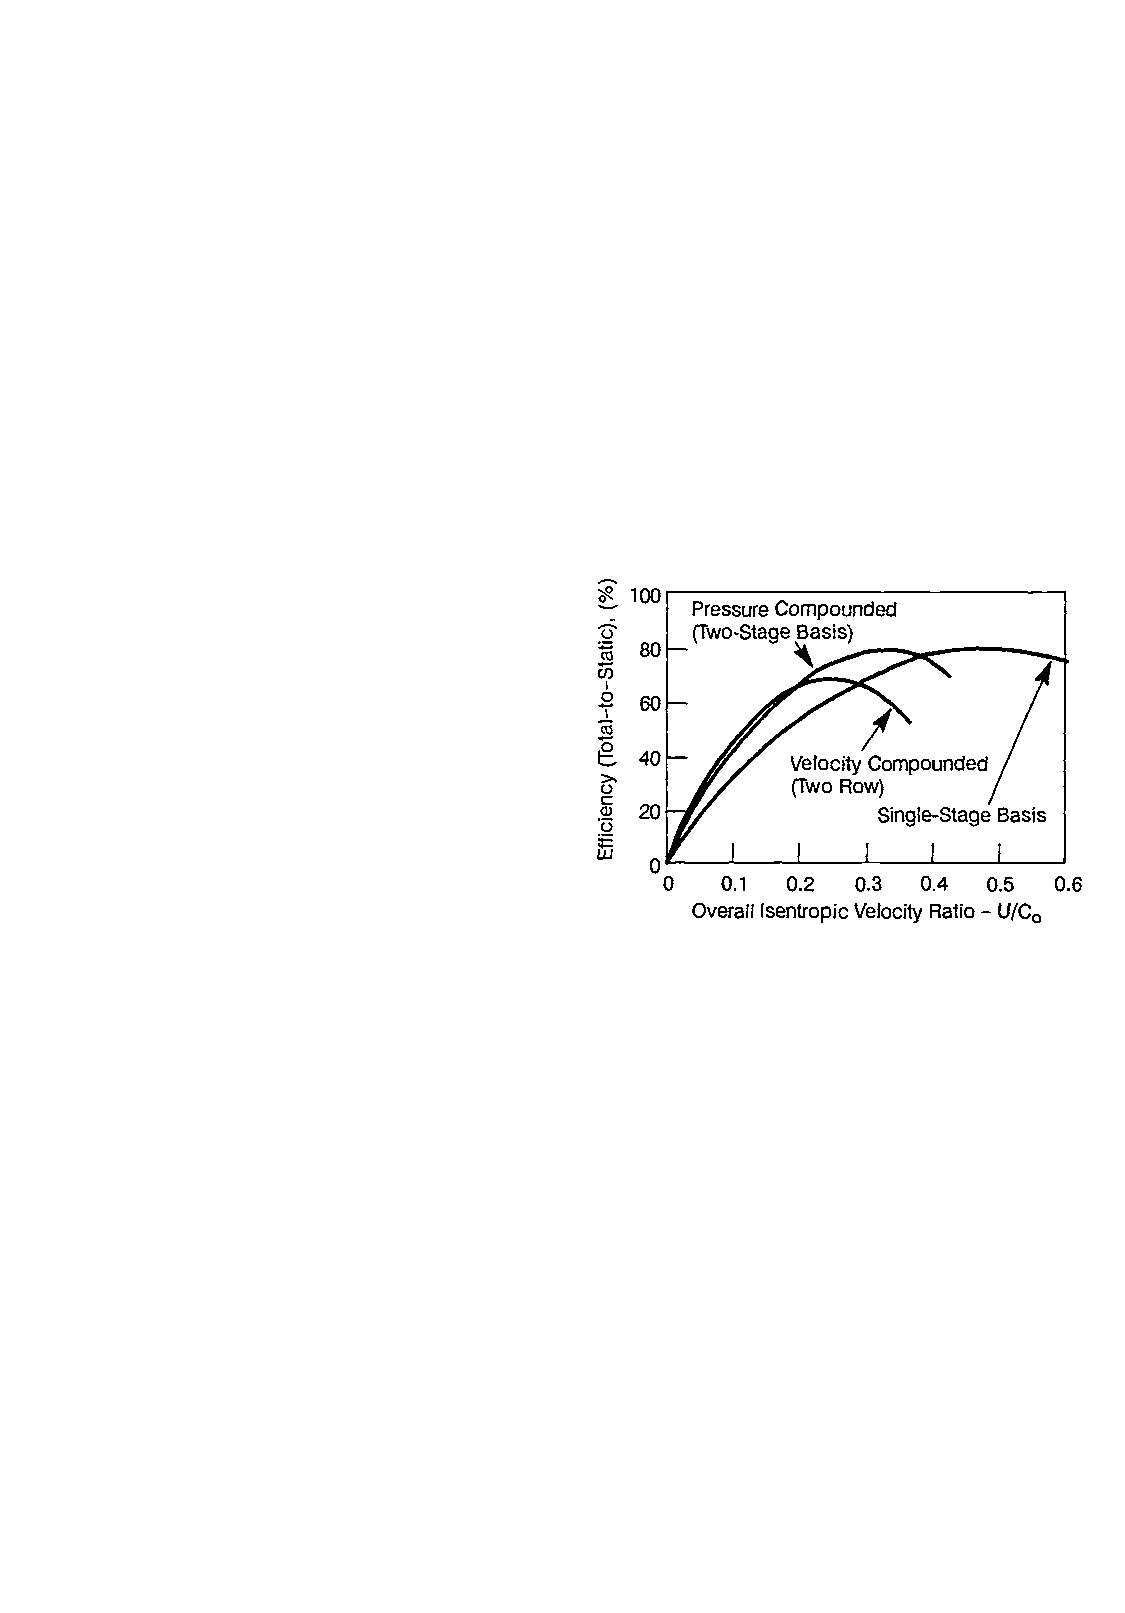
\includegraphics[width=\linewidth]{rendimenti_turbina}
	\caption{Rendimenti in funzione del rapporto di velocità}
	\label{fig:rendimenti_turbina}
\end{wrapfigure}

Questo valore è utile per capire la scelta progettuale effettuata per il tipo di turbina. Infatti, come già detto, nei cicli GG il salto di pressione in turbina è molto alto: questo implica un valore di $C_0$ elevato. Per avere una buona efficienza si possono percorrere più scelte progettuali (basandosi sul grafico x dei rendimenti). Si può scegliere di avere un alto rapporto di velocità con una singola ruota che 'assorba' tutta l'energia del flusso. Questo provocherebbe nel nostro caso una velocità di rotazione troppo elevata (quindi ingombro maggiore, inoltre la velocità di rotazione è fissata dalla pompa). Per usare altre turbine, cercando di avere un'alta efficienza si cerca di diminuire il rapporto di velocità aumentando gli stadi, ovvero la velocità del flusso è assorbita da più dischi che ruotano a velocità minori e sono più piccoli.

Le turbine PC (generano il salto di pressione in tutti gli statori) sono più efficienti ma più pesanti. Per cui si è optato per un sistema VC, che ha buona efficienza a bassi rapporti di velocità e permette un risparmio in peso.
}
\end{itemize}
\subsubsection{Analisi quantitativa - dimensionamento}

L'obiettivo ora è quello di cercare di dare un'idea a livello quantitativo dei vari componenti, generando un diagramma di velocità della turbina. 
Per questa sezione si sono presi in considerazione i requisti del sistema turbina, si sono ipotizzati diversi valori di rendimenti e sono state fatte alcune assunzioni ragionevoli per questo tipo di sistema (AIAA, modern engineering of LRE, Huzel ..). Abbiamo assunto i seguenti requisiti di sistema

\begin{table}[H]

\centering
\begin{tabular}{|c|c|c|c|c|c|}
\hline
$\bm{T_in \, [K]}$ & $\bm{p_in \, [bar]}$ & $\bm{\epsilon}$ &  $\bm{O/F}$ & $\bm{\dot{m} \, [kg/s]}$ & $\bm{\omega \, [rad/s]}$  \\
\hline
$1062$ & $67.57$ & $16.4$ &  $0.416$ & $75.75$ & $574.4$ \\
\hline
\end{tabular}

\caption{Requisiti del sistema turbina}
\label{table:turbine specs}

\end{table}

Assumendo tali dati, aggiungendo alcune ragionevoli ipotesi tratte dal libro AIAA e risolvendo il sistema di equazioni associato al problema, troviamo il seguente diagramma velocità e i corrispondenti valori di velocità e angoli. Si rimanda all'appendice per tutti i dettagli su ipotesi fatte, impostazione del sistema di equazioni e risoluzione del sistema tramite MATLAB.

%-----------------------------------------------------------------------------

\clearpage
\section{Piatto d'iniezione}
\label{sec:piatto iniezione}

\rfig{iniettore}{Piatto di iniezione}{iniettore}{0.4}

Gli iniettori sono collocati all’estremo superiore della camera di spinta e hanno lo scopo di distribuire il propellente in camera, regolando il rapporto di diluizione, la pressione e lo schema di spruzzo al fine di avviare e sostenere una combustione stabile. Per determinare questi valori sono stati necessari circa 3200 test su larga scala: al fine di generare un’esplosione controllata, risulta fondamentale che essa sia dinamicamente stabile, ossia che sia prevedibile e non crei punti caldi che porterebbero alla fusione di componenti del motore.

Il piatto di iniezione ha un diametro di 111.76 cm, è realizzato in CRES, acciaio molto resistente alla corrosione, ed è strutturato in 31 anelli, questi divisi in 13 scompartimenti da 2 deflettori circolari e 12 radiali. I vari compartimenti sono numerati da 1 a 13, mentre i deflettori sono identificati da lettere dalla A alla N.

La faccia del piatto di iniezione conta 1428 orifizi per l’ossidante e 1404 orifizi per il carburante. I getti vengono atomizzati attraverso una disposizione a doppietti omogenei, i vapori di combustibile e di ossidante si miscelano e reagiscono a formare i gas propellenti, destinati successivamente all’espansione in ugello.

Le 31 scanalature che costituiscono gli anelli consistono in 16 scanalature per il combustibile alternate alle 15 scanalature per l’ossigeno liquido. Gli anelli per il carburante sono alimentati attraverso un collettore radiale, mentre gli anelli per l’ossidante sono alimentati dal LOX dome tramite fori assiali.

Il LOX dome è considerabile il primo componente della camera di spinta: esso ha dimensioni 162.6 x 48.3 x 111.8 cm, con un peso di 818.3 kg; è realizzato in lega di ferro, rame e alluminio, con rivestimento in nichel e coating in silice. Il corpo del LOX dome contiene la flangia di attacco e i montanti di supporto per interfacciarsi con l’iniettore.

Il collettore invece incorpora due ingressi per il montaggio delle valvole di ossidante e una flangia per la linea di alimentazione dell’ossidante allo scambiatore di calore. Per evitare vorticità nell’ossidante, il collettore è isolato in due compartimenti da due argini toroidali. Solamente il 30\% del combustibile viene indirizzato direttamente al collettore, mentre il restante 70\% viene utilizzato per il raffreddamento rigenerativo della camera di spinta.

Sono inoltre presenti due alloggiamenti per gli ignitori del combustibile in ciascuno dei 12 scomparti esterni, e un alloggiamento del combustibile nel compartimento centrale, tutti collegati al collettore da singoli tubi di alimentazione.

Come detto precedentemente, è fondamentale ottenere una combustione stabile per non incorrere in danni alla camera di combustione: la stabilità è raggiunta principalmente mediante l’uso dei deflettori (baffles), oltre che variando l’angolo di impingement e il diametro degli orifizi in funzione della posizione sul piatto d’iniezione.

I deflettori in particolare alterano le caratteristiche acustiche di risonanza della camera di combustione, smorzando così le onde d’urto generate dalla combustione. I 12 deflettori radiali in rame sono alimentati dal deflettore circolare esterno. La configurazione dei deflettori utilizzata per il propulsore è stata ottenuta a seguito di vari test, nel quale si è ricercata la maggior stabilità di combustione possibile. Nella configurazione finale, i deflettori misurano circa 8 cm ciascuno e sono tutti dump-cooled, ovvero il raffreddamento è realizzato attraverso la circolazione di carburante all’interno del deflettore che viene successivamente scaricato nella camera di combustione. \cite{f-1_manual} \cite{JPP}

\begin{table}[H]

\centering
\begin{tabular}{|c|c|c|c|c|c|}
\hline
& $\bm{\dot{m} \, [kg/s]}$ & $\bm{A \, [m^2]}$ & $\bm{\Delta p \, [bar]}$ & $\bm{\rho \, [kg/m^3]}$ & $\bm{v \, [m/s]}$ \\
\hline
$\bm{fuel}$ & $742.09$ & $0.05484$ & $641$ & $810$ & $17.07$ \\
\hline
$\bm{oxidizer}$ & $1788.97$ & $0.03968$ & $2100$ & $1141$ & $40.54$ \\
\hline
\end{tabular}

\caption{Dati reali del piatto d'iniezione \cite{f-1_manual} \cite{JPP}}
\label{table:piatto iniezione}

\end{table}

A partire dai dati in \autoref{table:piatto iniezione}, è possibile inoltre stimare la velocità media teorica dei due propellenti all'uscita dai rispettivi iniettori:

\begin{empheq}{gather*}
	C_{D,f} = \frac{\dot{m}_{f}}{A_{f} \sqrt{2 \, \Delta p_{f} \, \rho_{f}}} = 13.28
	\qquad
	C_{D,ox} = \frac{\dot{m}_{ox}}{A_{ox} \sqrt{2 \, \Delta p_{ox} \, \rho_{ox}}} = 20.59
	\\
	v_{f} = C_{D,f} \sqrt{\frac{2 \, \Delta p_{f}}{\rho_{f}}} = 16.71 \, \text{m/s}
	\qquad
	v_{ox} = C_{D,ox} \sqrt{\frac{2 \, \Delta p_{ox}}{\rho_{ox}}} = 39.51 \, \text{m/s}
\end{empheq}

Tali risultati sono paragonabili alle velocità reali: la $v_{f}$ si discosta del 2.11\% dal valore reale, mentre la $v_{ox}$ si discosta del 2.54\%.

%-----------------------------------------------------------------------------

\section{Camera di spinta}
\label{sec:camera spinta}

\subsection{Descrizione del sistema}
\label{subsec:descrizione camera spinta}

L’intero gruppo della camera di spinta è costituito dal LOX dome, dal piatto di iniezione e dal corpo della camera di spinta.

In questa sezione verrà analizzato dettagliatamente il corpo della camera di spinta: esso è composto da una camera di combustione per bruciare propellenti seguita da un ugello di espansione a forma di campana, necessario ad espellere a velocità elevata i gas prodotti dai propellenti bruciati e poter così generare la spinta.

La camera di spinta è di circa 3.35 metri di lunghezza e 2.74 metri di diametro all'estremità inferiore dell'ugello. Il suo corpo è formato da tubi fino al piano in cui il rapporto di espansione diventa pari a 10:1; in questi scorre il 70\% del carburante, fornendo un raffreddamento rigenerativo ed evitando che il materiale del tubo si sciolga durante il funzionamento del motore.

I tubi che compongono la camera di spinta sono costruiti in Inconel X-750, una lega a base di nichel resistente alle alte temperature e trattabile termicamente, e sono rinforzati strutturalmente da una serie di fasce attorno all'ugello.

Il corpo sopra il piano corrispondente a rapporto di espansione 3:1 (circa 76.2 cm sotto il piano di gola) è costituito da 178 tubi primari con diametro esterno di 2.78 cm, mentre dal piano con rapporto di espansione 3:1 al piano a 10:1 si biforcano diventando 356 tubi secondari con diametro esterno di 2.54 cm.

Questa biforcazione è dovuta principalmente alla geometria dell'ugello e alle proprietà fisiche del materiale usato. La circonferenza di un ugello è minima in corrispondenza della gola mentre aumenta nella sezione di espansione: l'entità dell'aumento di circonferenza ottenibile con un numero fisso di tubi è quindi limitata da quanto questi ultimi possano essere lavorati per rastremazione. Quando si raggiunge il punto in cui la circonferenza non può essere ulteriormente aumentata con il numero prefissato di tubi si rende quindi necessario un giunto di biforcazione.

L’Inconel X-750 è stato scelto come materiale poiché forniva gli elevati rapporti forza-peso necessari per resistere ai requisiti di spinta del motore; inoltre, l'elevata resistenza di questa lega ha consentito la progettazione di tubi con sezioni di parete più sottili, con conseguente diminuzione del peso. Il design più sottile per i tubi fornisce anche un adeguato raffreddamento della camera di spinta, con circa due terzi del flusso totale di carburante che transita attraverso i tubi. Esso finisce poi in un collettore posizionato all'estremità inferiore della camera, da cui viene poi drenato da 4 porte di drenaggio posizionate a 90 gradi l'una dall'altra.

I gas di scarico della turbina, dopo essere passati attraverso lo scambiatore di calore, vengono convogliati al collettore di scarico della turbina, la cui funzione è quella di raccogliere e distribuire uniformemente il gas di scarico tra le pareti dell’estensione dell'ugello, che altrimenti non sarebbe raffreddato.

Le piastre divisorie all'ingresso e le alette di flusso nell'area di uscita contribuiscono alla distribuzione uniforme dei gas di scarico nell'estensione dell'ugello. Il collettore di scarico è saldato ad uno scudo ignifugo nella parete esterna della camera di spinta.

\subsection{Camera di combusione}
\label{subsec:camera_di_combustione}

Nel motore F-1 è presente una camera di combustione cilindrica con una parte finale convergente che termina con la sezione di gola.
La camera di combustione funge da involucro che deve mantiene i propellenti per un periodo sufficiente a garantire la completa miscelazione e combustione. Il tempo di permanenza richiesto, o tempo di residenza, è una funzione di molti parametri, ovvero combinazione di propellenti, le condizioni di iniezione e la geometria del combustore (rapporto di contrazione, numero di Mach, livello di turbolenza).

Un parametro utile relativo al volume della camera e il tempo di residenza è la "lunghezza caratteristica", L*, ossia il volume della camera diviso per l’area di gola:

FORMULEEEEE


Il concetto di L* è molto più facile da visualizzare rispetto al più elusivo "tempo di residenza", espresso in piccole frazioni di secondo, infatti si tratta di un sostituto per determinare il tempo di permanenza nella camera dei propellenti.

Un altro parametro fondamentale per il calcolo del tempo di residenza è la velocità caratteristica c*.
Il valore c* aumenta con L* fino a un massimo asintotico, ma l’aumento di L* oltre un certo punto tende a diminuire le prestazioni complessive del motore a causa di quanto segue: un maggiore L* si traduce in maggiore volume e peso della camera di spinta, con conseguente aumento della superficie che ha bisogno di raffreddamento e aumento delle perdite termiche e dovute all’attrito.
Il metodo abituale per stabilire la L* di un nuovo progetto della camera di spinta si basa in gran parte sull'esperienza passata con propellenti e dimensioni del motore simili. 
Nel caso della coppia di LOX/RP-1 la L* è compresa tra i valori 1÷1.30 metri, e per motivi progettuali descritti in precedenza è stata fissata la misura di L* a 1 m.
Partendo da questo dato e dalla dimensione dell’area di gola del motore è possibile modellare la camera di combustione.

Invertendo la formula della L* è possibile ottenere il volume della camera di combustione Vc che comprende, oltre alla parte cilindrica, anche la parte convergente.

FORMULAAAAAA

È possibile anche calcolare la velocità caratteristica c* e il tempo di residenza attraverso le seguenti due formule:

FORMULEEEEEE

Per calcolare le dimensioni reali di entrambe le parti della camera di combustione, ovvero la parte cilindrica e quella del convergente, è necessario fissare due parametri al fine dello sviluppo del modello.
Si tratta del rateo di contrazione, ossia il rapporto tra la sezione della camera cilindrica e la sezione di gola, e l’angolo di inclinazione del convergente

FORMULEEEEEEE

Sfruttando la trigonometria si ottiene la lunghezza assiale del tratto convergente e considerando quest’ultimo come una figura tronco conica si ottiene il volume da rapportare a quello calcolato in precedenza, così da ottenere il valore percentuale dell’ingombro del convergente, utilizzato nei calcoli seguenti.
Si ottiene così una camera di combustione con le seguenti misure:

TABELLAAAAAAAA


\subsection{Modellazione dell'ugello}
\label{subsec:modellazione ugello}

L’obiettivo principale che si persegue nella progettazione dell’ugello di un endoreattore è quello di ottenere una forma che minimizzi le perdite di spinta per un qualsiasi rapporto di espansione richiesto.

Si procede quindi ad illustrare il metodo ideato da Rao per una progettazione ottimale rispetto ad un ugello di forma tronco-conica, con lo stesso rapporto di espansione, preso da riferimento:

\begin{empheq}{equation*}
L_{con} = \frac{\left( \sqrt{\epsilon} - 1 \right) - R_t}{\tan {15\degree}}
\end{empheq}
\vspace{5pt}

dove $ R_t $ indica il raggio di gola dell’ugello e 15° è l’angolo standard di semi-apertura dell’ugello.

\vspace{5mm}

\rfig{ugello_TOP}{Definizioni geometriche}{ugello_TOP}{0.5}

La forma a campana ottimale può essere approssimata da una parabola inclinata grazie a considerazioni geometriche, permettendo anche di abbozzare velocemente una forma dell’ugello che contempla una perdita di prestazioni trascurabile a livello di spinta. Proprio per questo motivo, questa tipologia è anche chiamata ugello TOP (Thrust Optimized Parabolic) ed ha effettivamente trovato applicazione pratica nei vettori di lancio perché ha performance migliori quando sovra-espande a livello del mare (le pareti dell’ugello TOP aiutano a ritardare la separazione del flusso grazie ad un’elevata contropressione) rispetto ad un ugello ottimizzato perfettamente a campana. Inoltre, la forma dell’ugello varia in modo minimale in base ai propellenti usati e perciò una stessa famiglia di ugelli TOP può essere adattata per qualsiasi combinazione di ossidante e combustibile.

I parametri di partenza sono: il rapporto di espansione $ \epsilon $, il raggio di gola $ R_t $ e la percentuale di campana $ \%_{bell} $ che si vuole ottenere; quest’ultimo valore deve essere compreso tra il valore massimo di 85\%, a cui si raggiunge un livello di efficienza dell’ugello del 99\% e che può essere aumentato solo di un ulteriore 0.2\% con una percentuale di campana 100\%, e il valore minimo del 70\%, a cui si comincia ad ottenere un notevole degrado di prestazioni. Si ricavano quindi a cascata:

\vspace{5pt}
\begin{empheq}{alignat*=2}
& R_e = \sqrt{\epsilon} \, R_t		&\qquad		& \text{raggio della sezione d’efflusso}
\\
& L_{ugello} = \%_{bell} \frac{\left( \sqrt{\epsilon} - 1 \right) - R_t}{\tan {15\degree}}
&\qquad		& \text{lunghezza dell’ugello}
\end{empheq}
\vspace{5pt}

Si ricavano poi gli angoli $ \theta_n $, riferito al punto di inflessione N, e $ \theta_e $, riferito alla sezione d’uscita, per interpolazione grafica da curve analitiche ottenute sperimentalmente per determinati valori di $ \%_{bell} $ (grafico in \autoref{fig:angoli_bell}).

La prima parte di modellazione vera e propria consiste nella costruzione della gola dell’ugello secondo una geometria ottimale usata da Rao (ai tempi ingegnere alla Rocketdyne) e basata sull’intersezione di due archi di circonferenza definiti come segue:

\begin{empheq}{equation*}
x = 1.5 \, R_t \cos \theta	\qquad	y = R_t \left( 1.5 \, \sin \theta + 1.5 + 1 \right)
\end{empheq}

per la sezione di entrata, con $ -103\degree < \theta < -90\degree $ (l’angolo iniziale di -103° è scelto dal progettatore della camera di combustione \cite{nozzle_design} ma può anche essere fissato ad un valore differente);
\vspace{5pt}

\begin{empheq}{equation*}
x = 0.382 \, R_t \cos \theta	\qquad	y = R_t \left( 0.382 \, \sin \theta + 0.382 + 1 \right)
\end{empheq}

per la sezione di uscita, con $ -90\degree < \theta < \theta_n - 90\degree $.
\vspace{5mm}

Per la costruzione della campana è invece necessario definire prima tre punti geometrici:

\begin{itemize}[wide,itemsep=8pt,topsep=8pt]

\item
punto di inflessione N: $ \quad \text{N} = \begin{bmatrix} N_x \\ N_y \end{bmatrix} = \begin{bmatrix}
0.382 \, R_t \cos \left( \theta_n - 90\degree \right) \\
R_t \left[ 0.382 \, \sin \left( \theta_n - 90\degree \right) + 0.382 + 1 \right]
\end{bmatrix} $
\item
punto tangente alla sezione d'efflusso E: $ \quad \text{E} = \begin{bmatrix} E_x \\ E_y \end{bmatrix} = \begin{bmatrix} R_e \\ L_{ugello} \end{bmatrix} $
\item
punto Q di intersezione delle rette passanti da N con inclinazione $ \theta_n $ e da E con inclinazione $ \theta_n $:

\begin{empheq}{alignat*=2}
&\overrightarrow{NQ} = m_1 x + C_1 \; \text{con} \; m_1 = \tan \theta_n \; \text{e} \; C_1 = N_y - m_1 N_x
&\qquad
& Q_x = \frac{C_2 - C_1}{m_1 - m_2}
\\
&\overrightarrow{QE} = m_2 x + C_2 \; \text{con} \; m_2 = \tan \theta_e \; \text{e} \; C_2 = E_y - m_2 E_x
&\qquad
& Q_y = \frac{m_1 C_2 - m_2 C_1}{m_1 - m_2}
\end{empheq}

\end{itemize}
\vspace{5pt}

La campana infine risulta essere una curva di Bézier quadratica di equazione:

\begin{empheq}{alignat*=2}
& x(t) = \left( 1 - t \right)^2 N_x + 2 \left( 1 - t \right) t \, Q_x + t^2 E_x &\qquad
& 0 \le t \le 1 \\
& y(t) = \left( 1 - t \right)^2 N_y + 2 \left( 1 - t \right) t \, Q_y + t^2 E_y &\qquad
& 0 \le t \le 1
\end{empheq}

\vspace{5pt}
\subsection{Cooling della camera di spinta}
\label{subsec:cooling camera}

I motori a propellente liquido sfruttano varie tecnologie per il raffreddamento delle pareti della camera di spinta. Nel caso analizzato, il motore F-1 sfrutta due tipi di raffreddamento: il film cooling, che protegge le pareti dell'estensione dell'ugello attraverso un sistema di iniezione, e il raffreddamento rigenerativo, che utilizza il combustibile come fluido refrigerante passante attraverso una serie di tubi che costituiscono la parete stessa dell'ugello.

\subsubsection{Scambio termico convettivo e film cooling}

Per poter analizzare la protezione termica delle pareti della camera di spinta, è in primo luogo necessario stimare il valore di scambio termico convettivo dai gas combusti alle pareti stesse.

La trattazione dello scambio termico convettivo nel caso preso in analisi viene affrontata tenendo conto dalle alte velocità dei gas combusti: ciò porta alla formazione di uno strato limite, che si assottiglia lungo il convergente in concomitanza con l'accelerazione del fluido subsonico, raggiungendo il minimo in gola, per poi ispessirsi nel divergente. Lo scambio termico è quindi un problema riguardante lo strato limite e il suo spessore, la sua temperatura e la velocità del fluido.IMMAGINE.

Poichè si raggiunge il minimo spessore dello strato limite in gola, ci si aspetta di avere il massimo scambio convettivo nel punto dell'ugello in cui il rapporto $A_t$ su A è minimo. Questa osservazione è di particolare rilevanza, poiché, come si vedrà più avanti, per determinare la portata massica necessaria per il film cooling, si utilizzerà l'area della sezione minima dell'estensione dell'ugello, che corrisponde all'area della sezione con rapporto di espansione 10:1.

Risulta complicato determinare il valore preciso del calore scambiato in modo convettivo tra i gas combusti e le pareti, in quanto lo strato limite è fortemente influenzato da vari fattori, quali la curvatura delle pareti, il gradiente di pressione in direzione assiale, il gradiente di temperatura associato all'alta intensità del flusso di calore; è tuttavia possibile utilizzare un metodo semi-empirico per farne una accurata stima.

Lo scambio convettivo per unità di area lato gas all’interfaccia tra fluido e superficie solida dipende da un coefficiente detto "coefficiente di film" $h_g$ : FORMULA CON \[ASTERISCO\] PERCHE RIPRESA ALLA FINE DELLA TRATTAZIONE
dove $T_{wg}$ è la temperatura della parete dal lato caldo, mentre $T_{aw}$ è la temperatura adiabatica della parete. Per determinare la temperatura $T_{wg}$ è sufficiente moltiplicare la temperatura in camera di combustione per un fattore pari a 0.8, fattore che tiene conto della presenza di depositi solidi di carbonio sulle pareti.

Per comprendere il significato della temperatura adiabatica $T_{aw}$ è necessaria una piccola digressione. La velocità del fluido all'esterno dello strato limite è la velocità del flusso libero e, attraversando lo strato limite perpendicolarmente alla parete, la velocità diminuisce fino ad annullarsi per soddisfare la condizione di aderenza. La temperatura a parete dovrebbe perciò essere pari alla temperatura di ristagno, ossia la temperatura raggiunta quando tutta l'energia cinetica viene trasformata in energia termica senza alcuna perdita. Nel caso di flussi molto veloci, l'aumento di temperatura è abbastanza elevato da provocare un processo di rallentamento viscoso non adiabatico. Per questo motivo, nell'ipotesi di parete adiabatica verso l'esterno, avviene un significativo scambio termico dal fluido in prossimità della parete, caratterizzato da bassa velocità e alta temperatura statica, verso il fluido più lontano dalla parete. A parete si avrà quindi una temperatura $T_{aw}$ più bassa della temperatura che caratterizza il flusso libero, mentre all'interno dello strato limite, affinché venga soddisfatta l'equazione dell'energia per flussi stazionari, deve essere necessariamente presente una regione in cui la temperatura è più alta di quella del flusso libero. Si delinea un andamento della temperatura come schematizzato in figura. IMMAGINE

Nel caso preso in esame, il valore della temperatura $T_{aw}$ è determinabile scalando la temperatura in camera di combustione di un fattore detto "recovery factor" $f_{aw}$ , definito come legame tra $T_{aw}$ e le temperature statica e totale del flusso libero e con valore compreso tra 0.9 e 0.98. In particolare il recovery factor rappresenta il rapporto tra l'aumento della temperatura causato dall'attrito e l'aumento causato dalla compressione adiabatica. Esso è determinabile sperimentalmente o può essere stimato in base ad una correlazione semplificata e applicata nel caso di flusso turbolento, basata sul numero di Prandtl: FORMULA (Pr elevato 0.33), dove il numero di Prandtl può essere approssimato come segue: FORMULA + VALORE DI MU.

È necessario precisare che la temperatura in camera di combustione $T_c$ utilizzata è quella teorica moltiplicata per il fattore correttivo della velocità caratteristica. Quest'ultima infatti dipende unicamente dalla variabile $T_c$, quindi il fattore correttivo per le due grandezze coincide. Il suddetto fattore varia in un intervallo compreso tra 0.87 e 1.03, mentre il valore utilizzato nella trattazione, ossia 0.975, è il valore sperimentale adottato dal libro Modern Engineering for Design of Liquid Rocket Propellant.

Per stabilire il valore di calore scambiato per unità di area rimane da calcolare solo il coefficiente di film $h_g$, che può essere ricavato mediante la seguente formula: FORMULA
dipendente, tra gli altri parametri, dal numero di Prandlt, dalla viscosità, dal raggio di curvatura in gola dell'ugello e dal fattore correttivo SIGMA, che tiene conto delle variazioni di proprietà attraverso lo strato limite. 
Il raggio di curvatura in gola dell'ugello è stato ricavato tramite approssimazione di Rao. 
L'unico valore incognito è quindi SIGMA: questo fattore può essere determinato in termini di temperatura di combustione, temperatura locale a parete e numero di mach locale mediante la relazione di Bartz; in alternativa è possibile determinarlo per interpolazione, in funzione del rapporto $T_{wg}$ DIVISO $T_c$ e del valore di GAMMA. IMMAGINE. Assumendo il rapporto $T_{wg}$ DIVISO $T_c$ pari a 0.8, ricavato sperimentalmente e adottato nella trattazione nel volume Liquid Rocket Engine e che tiene conto della presenza del deposito di carbonio sulle pareti, noto il valore di GAMMA, pari a 1.2439, e ricordando che il fine ultimo del calcolo è progettare il film cooling dell'ugello aggiuntivo (intervallo di rapporto di espansione 0.1 - 1.6), è possibile determinare dal grafico che il valore del fattore correttivo si attesta intorno a 0.7 in tutto l'intervallo in esame.
Il coefficiente di film dipende infine anche dal rapporto $A_f$ su A, dove A è l'area della sezione locale. Il valore di questo rapporto è stato fatto variare per via numerica tra 0.1 e 1.6, calcolando poi per ciascun valore il corrispondente coefficiente di film e, in seguito, la corrispondente portata minima in massa per effettuare un adeguato film cooling.
Il valore di $h_g$ così ottenuto tiene unicamente in conto del calore scambiato tra fluido e parete, senza considerare la presenza di eventuali prodotti di combustione allo stato solido. I prodotti di combustione della coppia LOX – RP-1 contengono circa lo 37 in percentuale di particolato solido. Queste particelle tendono a depositarsi sulle pareti della camera di combustione, formando un efficace strato isolante: la valutazione quantitativa dell’efficacia dell’isolamento di questo strato, necessaria per il corretto calcolo dello scambio di calore, può essere effettuata solo sperimentalmente. Lo strato isolante è formato a sua volta da uno strato superficiale di fuliggine, che ne sovrasta uno piu tenace: quest’ultimo aumenta la resistenza termica lato gas, tale che la temperatura del deposito di carbonio all’interfaccia lato gas si avvicini alla temperatura del gas all’aumentare dello spessore del layer di carbonio.
Per il calcolo dello scambio termico nel caso di presenza di deposito solido sulle pareti della camera, l’equazione [ASTERISCO] viene corretta dalla seguente equazione, che vede una sostituzione del coefficiente di film con il coefficiente di conduttanza termica complessiva lato gas $h_{gc}$ FORMULA
Questo coefficiente considera sia $h_g$ sia il coefficiente di resistenza causata dal deposito solido $R_d$ , il cui valore è dipendente dal rapporto di espansione e dalle condizioni di pressione e rapporto di miscela FORMULA
Dopo aver calcolato tutti i parametri necessari, è quindi possibile progettare il sistema di film cooling dell'estensione dell'ugello. Il film cooling delle pareti interne è ottenuto iniettando i gas di scarico della turbina, forniti alla cavità tra le pareti dal collettore di scarico della turbina, nel flusso di scarico della camera di spinta attraverso fessure formate da 23 file di scandole sovrapposte che formano la parete interna.
Per lo sviluppo dei calcoli si consideri che il fluido di lavoro è gas con presenza di particolato, ed è quindi possibile utilizzare la relazione di Hatch e Papell, sostituendo al coefficiente $h_g$ il coefficiente $h_{gc}$ appena calcolato FORMULA
ove $T_{co}$ è la temperatura iniziale del fluido refrigerante, ossia la temperatura all'uscita dello scambiatore; $C-{pvc}$ è il calore specifico medio a pressione costante del fluido refrigerante, che è stato numericamente ottenuto interpolando i valori dopo la turbina in frozen equilibrium; infine $NU_{c}$ è l'efficienza del film cooling ed è un fattore che ha scopo correttivo, ossia tiene conto della quantità di refrigerante gassoso perso nel flusso di gas di combustione che quindi non produce effetti di raffreddamento. I valori dell'efficienza variano dal 25 al 65 in percentuale in funzione della geometria dell'iniezione del refrigerante e dalle condizioni di flusso. 
Dalla precedente equazione si evince che l'apporto termico dipende dal coefficiente di scambio $h_gc$ e dalla differenza tra temperatura adiabatica a parete e la temperatura del refrigerante; il calore assorbito è proporzionale alla capacità termica del film refrigerante dal valore di temperatura iniziale a quello finale. Esiste quindi un equilibrio tra apporto di calore e aumento di temperatura del refrigerante: raggiunto questo equilibrio si raggiunge la condizione adiabatica e la superficie della parete avrà localmente la medesima temperatura del film; infatti la temperatura della parete varierà assialmente dalla temperatura iniziale del refrigerante fino alla temperatura massima ammissibile.
L'obiettivo del calcolo è perciò quello di determinare la portata massica di fluido refrigerante per unità di area $G_c$, che poi verrà moltiplicato per l'area dell'estensione dell'ugello ad ottenere il valore di portata massica necessaria per il film cooling. Si noti che la portata dipende dal valore $h_{gc}$ , a sua volta dipendente dal rapporto $A_t/A$, che è stato fatto variare tra 1:10 e 1:16 : la portata massica che sarà sufficiente a raggiungere un efficiente film cooling in ogni sezione dell'ugello sarà la portata massima tra le portate calcolate, ossia quella ottenuta per rapporto $A_t$ su A maggiore e perciò A minore, quindi l'area della sezione 1:10. Il valore di Gc ottenuto è minore della portata elaborata dal gas generator, e questo è un risultato prevedibile in quanto il valore di portata passante per il gas generator è dettato dai requisiti di potenza della turbina e non dalle esigenze del film cooling. È stato perciò dimostrato che la portata massica elaborata è sufficiente a raggiungere l'obiettivo desiderato di raffreddamento delle pareti.

\subsubsection{Regenerative cooling}
\label{subsubsec:regenerative cooling}

Il motore preso in esame sfrutta lo scambio termico rigenerativo come tecnica di raffreddamento delle pareti della camera di spinta, in particolare dalla gola e per la lunghezza dell'ugello fino al piano caratterizzato da rapporto di espansione 10:1. Il regenerative cooling utilizza una quota parte di combustibile stivato, circa il 70 per cento, come refrigerante: esso viene indirizzato in una serie di tubi opportunamente sagomati saldobrasati insieme che costituiscono la parete stessa dell'ugello di efflusso. Lo scambio di calore avviene quindi tra due flussi in movimento separati da una parete.
Questa tecnica vanta di alcuni importanti vantaggi, tra i quali il fatto che non comporti nessuna perdita di prestazioni, infatti l'energia termica assorbita del refrigerante viene restituita all'iniettore, e abbia una struttura relativamente leggera. Tuttavia si possono riscontrare alcuni svantaggi, come alte perdite di pressione per elevati livelli di flusso di calore.

La seguente figura IMMAGINE descrive la variazione di temperatura durante lo scambio di calore per regenerative cooling: a sinistra scorrono i gas combusti a contatto con il boundary layer e la cui temperatura è $T_{aw}$ (il cui significato è illustrato nel sottoparagrafo precedente), ossia la temperatura che verrebbe raggiunta dalla parete nel caso di parete adiabatica o isolante, che diminuisce sensibilmente all'interno del boundary layer fino a raggiungere la temperatura della parete lato gas $T_{wg}$. All'interno dello spessore della parete la temperatura continua a diminuire raggiungendo la temperatura $T_{wc}$, ossia la temperatura della parete a contatto con il refrigerante; quest'ultimo quindi sarà caratterizzato dalla temperatura $T_{c0}$ (bulk temperature del refrigerante).

Proprio a causa dello scambio di calore tra gas e refrigerante, la temperatura $T_{c0}$ aumenterà dal punto di ingresso fino al momento in cui l'RP-1 lascerà il condotto di raffreddamento: essa è quindi una funzione del calore assorbito e della portata. A livello strutturale è necessario svolgere il dimensionamento nel punto più critico, ossia nel tubo di ritorno all'altezza della gola, ossia l'ultima sezione attraversata dal refrigerante prima di essere immesso nella camera di spinta.

L'obiettivo ultimo del regenerative cooling è quello di mantenere la temperatura della parete al di sotto della temperatura critica alla quale possono realizzarsi fusioni localizzate o un decremento delle prestazioni del materiale. La temperatura limite nel caso della parete della camera di spinta dell'F-1, realizzata in Inconel X750, è tra 1100 K e 1255 K.
Identificate le temperature caratteristiche del processo di raffreddamento è quindi possibile calcolare il flusso di calore come: FORMULA

Rimaneggiando la formula essa può essere riscritta in funzione del coefficiente globale di scambio termico FORMULE
dove $h_{gc}$ è la conduttività termica complessiva lato gas, $h_{c}$ è il coefficiente di scambio termico lato refrigerante, mentre t è lo spessore della parete e k la conduttività termica della parete della camera. Osservando la precedente equazione è possibile introdurre un ulteriore requisito che il regenerative cooling deve soddisfare: per mantenere la temperatura della parete entro valori contenuti, è necessario che la conduttività termica complessiva lato gas $h_{gc}$ sia minimizzata, mentre il coefficiente di scambio termico del refrigerante sia molto alto, cosi come il rapporto t DIVISO k. Dal momento che la differenza di temperatura è inversamente proporzionale al coefficiente di scambio termico del flusso di calore, la diminuzione della temperatura sarà più rapida tra gas caldo e parete interna della camera.

Se per determinare il valore di $h_{gc}$ è sufficiente ripercorrere la trattazione riguardante lo scambio termico convettivo, per comprendere il significato del coefficiente $h_c$ e determinarne il valore numerico è necessario approfondire il suo legame con pressione e temperatura critica del refrigerante.
IMMAGINE Verranno analizzati due possibili scenari, rappresentati in figura: la curva $A_i$ descrive l'andamento del legame temperatura della parete – flusso di calore nel caso di pressione minore della pressione critica mentre la curva $B_i$ rappresenta l'andamento del legame nella condizione di pressione maggiore della pressione critica.

Studiando la curva A, il tratto A1-A2 rappresenta lo scambio di calore nelle condizioni in cui la temperatura della parete lato coolant non ha ancora raggiunto la temperatura di saturazione, in corrispondenza della pressione del refrigerante. Alla temperatura del punto A2, superata la temperatura di saturazione, il combustibile inizia a bollire, creando quindi delle “bolle” nella fascia a ridosso della parete. Queste crescono di dimensione nel flusso liquido piu freddo fino a che la velocità di condensazione del vapore supera la velocità di vaporizzazione: le bolle iniziano a collassare. Questo processo, che avviene ad alta frequenza, è detto “Nucleate boiling” (ebollizione nucleata). In corrispondenza di questo fenomeno il coefficiente di scambio termico aumenta, causando un aumento contenuto della temperatura a parete per un'ampia gamma di flussi di calore. Lo scambio di calore caratterizzato da ebollizione nucleata è rappresentato dal tratto A2-A3. Alla temperatura corrispondente al punto A3, un ulteriore aumento del flusso di calore porta ad un incremento di concentrazione di bolle tale per cui esse si combinano in un film di vapore a cui consegue una forte diminuzione del coefficiente del trasferimento del calore (tratto A3-A4). Lo scambio di calore raggiunto al punto A3 definisce il limite superiore del nucleate boiling, valore che viene quindi utilizzato come limite di progetto per il sistema di raffreddamento rigenerativo.
La curva B descrive le varie fasi del legame flusso di calore- temperatura della parete nel caso in cui la pressione sia al di sopra di quella critica: in queste condizioni di il fenomeno di nucleate boiling non si manifesta. Queste condizioni portano ad un aumento di temperatura proporzionale all'incremento del flusso di calore: in questo modo si raggiunge la temperatura limite per un valore di scambio di calore minore. Per questo motivo si predilige una pressione che sia tra il 30 e il 70 in percentuale della pressione critica.
Il dimensionamento del sistema di regenerative cooling è finalizzato a stabilire il numero di tubi che compongono la parete dell'ugello d'efflusso e le dimensioni dei singoli tubi, in particolare il diametro interno e lo spessore. Prima di procedere alla trattazione matematica è necessario chiarire alcune assunzioni considerate durante lo svolgimento dei calcoli. Il dimensionamento viene effettuato nella condizione piu critica, ossia vengono dimensionati i tubi di ritorno nella sezione di gola, perché la gola rappresenta il punto caratterizzato dal maggior valore di flusso termico attraverso e attraverso la sezione finale dei tubi di ritorno scorre il refrigerante alla sua temperatura massima raggiunta dopo aver percorso tutto il sistema di raffreddamento; la forma dell'ugello d'efflusso fa fede alla modellazione illustrata precedentemente e viene perciò considerata nota: dalla modellazione e dalla simulazione RPA verranno ricavati il diametro di gola e i raggi di curvatura utili a determinare il raggio di curvatura medio R; il numero di tubi rimane costante fino al piano caratterizzato dal rapporto di espansione 3:1, per poi raddoppiare fino al piano con rapporto di espansione 10:1. Infine, avendo come variabili sia il numero di tubi sia il loro spessore, è necessario ipotizzare o fissare uno dei due dati: è stato quindi fissato il numero reale di tubi che compongono l'ugello nel primo tratto, ossia 178, mantenendo come incognita lo spessore.
I calcoli preliminari al dimensionamento permettono di determinare, tramite una trattazione analoga a quella illustrata per lo scambio convettivo, il valore di flusso di calore specifico q, funzione della conduttività termica, della temperatura adiabatica a parete e della temperatura della parete lato gas. 
La temperatura a parete lato gas $T_{wg}$ è determinata sperimentalmente (Modern Engineering), mentre la temperatura adiabatica a parete $T_{aw}$ è ottenuta moltiplicando la temperatura in camera di combustione $T_c$ per il fattore di recupero dello strato limite turbolento in gola (valore intermedio tra 0.9 e 0.98). Noto quindi il rapporto $T_{wg}$ DIVISO $T_c$ e il gamma dei gas combusti è possibile determinare il valore del fattore di correzione in gola sigma dai grafici riportati nella sezione precedente. Infine è possibile calcolare il coefficiente di scambio termico lato gas tramite la formula: FORMULA
e quindi il valore della conduttività termica lato gas FORMULA
IMMAGINE A LATO Dalle precedenti formule è possibile definire $R_d$ la resistenza termica causata dal deposito solido in gola, R il raggio di curvatura dell'ugello calcolato come media dei due raggi di curvatura $R_1$ ed $R_n$, $D_t$ il diametro di gola calcolato come due volte $R_t$.
Terminati i calcoli preliminari è possibile passare al dimensionamento vero e proprio del sistema di refrigerazione. Sono noti i valori relativi alla lega X750 (conducibilità termica $k_lega$, modulo di elasticità E, coefficiente di espansione termica a, coefficiente di Poisson v) e vengono assunti i valori di bulk temperature del combustibile in gola, la sua conducibilità termica $k_fuel$, la sua densità (di stivaggio) e una costante $C_1$ propria dell’RP1 utile per il calcolo del numero di Nusselt (valore adottato dalla trattazione del volume Modern Engineering)
A questo punto per determinare lo spessore t dei tubi è possibile implementare un ciclo for che permetta di calcolare il numero dei tubi al variare dello spessore, per poi interrompere il ciclo quando il numero eguaglia il numero di tubi imposto: in questo modo si ottiene il valore dello spessore necessario. I calcoli svolti si basano su considerazioni fisiche e su formule empiriche.
Il ciclo inizia con il calcolo della temperatura della parete lato combustibile FORMULA necessario per determinare il valore del coefficiente  di scambio termico del combustibile FORMULA.
Per regioni di temperatura subcritica caratterizzate dall'assenza di nucleate boiling, la relazione tra temperatura a parete e flusso di calore, che dipende per l'appunto dal coefficiente di scambio termico $h_c$, può essere descritto tramite l'equazione di Sieder-Tate per il trasferimento di calore turbolento ai liquidi che fluiscono nei canali: FORMULA
dove mu è la viscosità del combustibile alla temperatura $T_{co}$, mentre $mu_w$ è la viscosità del combustibile alla temperatura della parete in gola. Questa relazione può essere riscritta esplicitando i singoli termini: FORMULA \[1 ASTERISCO\]
ove le incognite sono il diametro dei tubi d e la velocità media del combustibile $V_co$. Quest'ultima può essere calcolata in funzione del diametro dei tubi e del loro numero FORMULA
con $W_f$ la portata massica di combustibile, corrispondente al 70 per cento della portata totale del combustibile.
Tramite una formula empirica è possibile esplicitare l'espressione che permette di definire il numero di tubi FORMULA \[2 ASTERISCHI\].
Il fattore 0.8 ha il ruolo di fattore di correzione: il centro dei tubi è collocato su una circonferenza, piuttosto che su una retta.
Sostituendo quindi $V_{co}$ all'interno dell'equazione (1 ASTERISCO) esplicitandone N ed eguagliando l'espressione trovata all'equazione (2 ASTERISCHI) è possibile determinare il valore del diametro dei tubi. Sostituendo infine il valore trovato all'interno dell'equazione (2 ASTERISCHI) il si ottiene il numero dei tubi. Analizzando in un ciclo for i passaggi appena visti, è possibile determinare il valore di t tale per cui si ha il numero di tubi N desiderato.

\subsection{Confronto tra ugello 10:1 e 16:1}
\label{subsec:confronto ugello}

I motori F-1 prodotti dalla Rocketdyne avevano in origine un ugello il cui rapporto di espansione era 10:1; essi infatti non furono inizialmente progettati nello specifico per lo stadio di lancio del Saturn V. Gli ingegneri decisero quindi a posteriori di aggiungere un'espansione dell'ugello iniziale allo scopo di migliorare vari parametri del lanciatore: i più rilevanti sono l'impulso specifico nel vuoto e la quota a cui è raggiungibile l'espansione ottima (adattata alla traiettoria che il lanciatore avrebbe percorso).

Tale espansione non poteva essere raffreddata dal già presente regenerative cooling: si optò dunque per una soluzione che prevedesse l'utilizzo dei gas di scarico della turbina, ricchi di carbonio e quindi con bassa conducibilità termica, per il raffreddamento attraverso film cooling. Tale tipo di raffreddamento è realizzato immettendo i gas di scarico sulle pareti dell'ugello attraverso un collettore che ne abbraccia l'intera circonferenza.

L'estensione dell'ugello è realizzata da due pareti in lega di nickel intervallate da bande circolari in CRES: tale costruzione saldata conferisce ottima resistenza termica alle pareti e una buona resistenza agli sforzi radiali a cui l'ugello è sottoposto.

Di seguito sono confrontati i principali parametri del motore con e senza l'espansione dell'ugello, ricavati tramite il software RPA:

\begin{table}[H]

\centering
\begin{tabular}{|c|c|c|c|c|c|c|}
\hline
& $\bm{p_e \, [bar]}$ & $\bm{T_e \, [K]}$ & $\bm{H \, [kJ/kg]}$ & $\bm{\gamma}$ & $\bm{\rho \, [kg/m^3]}$ & $\bm{v_e \, [m/s]}$ \\
\hline
\textbf{10:1} & $0.803$ & $1673.7$ & $-5058.1$ & $1.2439$ & $0.1304$ & $2910.6$ \\
\hline
\textbf{16:1} & $0.423$ & $1473.0$ & $-5429.9$ & $1.2521$ & $0.0781$ & $3035.6$ \\
\hline
\end{tabular}

\vspace{5pt}

\begin{tabular}{|c|c|c|c|c|c|c|}
\hline
& $\bm{I_{vac} \, [s]}$ & $\bm{I_{opt} \, [s]}$ & $\bm{I_{sl} \, [s]}$ & $\bm{T_{vac} \, [kN]}$ & $\bm{T_{opt} \, [kN]}$ & $\bm{T_{sl} \, [kN]}$ \\
\hline
\textbf{10:1} & $297.36$ & $276.44$ & $270.95$ & $7816.3$ & $7266.3$ & $7122.2$ \\
\hline
\textbf{16:1} & $306.25$ & $288.59$ & $263.99$ & $8050.0$ & $7585.9$ & $6939.3$ \\
\hline
\end{tabular}

\caption{Confronto tra ugello 10:1 e 16:1}
\label{table:confronto_ugello}

\end{table}

Si può notare un miglioramento nella spinta e nell'impulso specifico in corrispondenza dell'espansione ottima e dell'espansione nel vuoto, mentre si ha un calo di prestazione a livello del mare: ciò è dovuto al fatto che l'ugello sovraespande in maniera più marcata a pressione standard, poiché il punto di espansione ottima viene spostato a pressioni inferiori. Ciò non risulta essere un problema in quanto la spinta rimane sufficiente al lancio, mentre i benefici ottenuti alle quote di missione sono rilevanti.

%-----------------------------------------------------------------------------
% APPENDICE
%-----------------------------------------------------------------------------

\clearpage
\addcontentsline{toc}{section}{Appendice}
\begin{appendices}

\section{Immagini e schemi}
\label{appendix:immagini}

\cfig{angoli_bell}{Grafico di interpolazione degli angoli per la costruzione dell'ugello}{angoli_bell}{0.8}

\section{Grafici di varie grandezze in funzione del tempo di volo}
\label{appendix:grafici volo}

\twofig{03_accelerazione_t}{Accelerazione in funzione del tempo}{accelerazione_t}{05_drag_t}{Drag in funzione del tempo}{drag_t}

\twofig{06_massa_t}{Massa totale in funzione del tempo}{massa_t}{08_gravita_t}{Accelerazione di gravità in funzione del tempo}{gravita_t}

\twofig{09_pressione_t}{Pressione ambientale in funzione del tempo}{pressione_t}{10_temperatura_t}{Temperatura ambientale in funzione del tempo}{temperatura_t}

\cfig{11_mach_t}{Numero di Mach in funzione del tempo}{mach_t}{0.48}

\section{Confronto peso molecolare gas generator tra caso Fuel Rich e Oxidizer Rich}
\label{appendix:confronto_peso_molecolare}

Per poter apprendere come l'O/F influisca sulla massa molare dei prodotti si è utilizzato il software NASA CEA (CEAM \cite{CEAM_guide}). Si è utilizzato un problema HP, in modo da far raggiungere l'equilibrio chimico senza bloccarlo imponendo una temperatura (il problema HP di NASA CEA, con il GG, tende a sovrastimare la temperatura raggiunta come si vedrà in \autoref{appendix:prodotti_gas_generator}). La temperatura di equilibrio in questo caso è un parametro importante poichè in uscita dal GG abbiamo il vincolo della palettatura di turbina. Si è imposto che la temperatura in uscita dal GG debba essere minore di 1500K sia in FR che OR.  Si è fatto variare l'O/F da nel range $0.2 / 18$, si sono plottati i grafici di MM, T, $c_p$ in funzione dell'O/F.

\twofig{MM_to_OF}{Massa Molare prodotti in funzione di O/F}{MM_to_OF}{temperatura_gg_of}{Temperatura in uscita dal GG in funzione di O/F}{temperatura_gg_of}

Dal primo grafico si nota come ad O/F bassi (fuel rich mixture) si ottenga una massa molare media più bassa rispetto a miscele oxidizer rich. La zona compresa tra le due linee tratteggiate nere, nel primo grafico, non deve essere considerata poichè ad essa sono associate temperature troppo elevate per la turbina, come si nota nel grafico immediatamente a destra. 
Un altro vantaggio dato dalle miscele FR è che il valore di $c_p$ è più alto che nel caso OR. Questo permette di ottenere un lavoro specifico della turbina maggiore con le miscele FR. Infatti:

\begin{empheq}{gather*}
\Delta h_{id} = c_p \left( 1 -  \epsilon^{\frac{1 - \gamma}{\gamma}} \right) 
\end{empheq}
\vspace*{2.5mm}

Tale valore è influenzato principalmente dal valore di $c_p$ (oltre che dal valore di $\gamma$). Il calore specifico a pressione costante diminuisce, aumentando il rapporto O/F (per O/F > 3) \autoref{fig:c_p_gg}, per cui si ha una variazione di lavoro specifico rispetto all'O/F, come mostra il grafico \autoref{fig:delta_h_id}. I valori interessanti sono sempre quelli che rispettano il vincolo di temperatura, quindi relativi ad O/F minori di 1 e maggiori di 14. Notiamo inoltre che i grafici di $c_p$ e di $\Delta h_{id}$  hanno andamenti simili, per cui la variazione di $\gamma$ rispetto a O/F influenza poco l'andamento  di $\Delta h_{id}$ rispetto a $c_p$ nella formula C1. Questo perchè $\gamma$ varia nell'intorno dell'unità su tutto l'intervallo considerato \autoref{fig:gamma_gg}

\twofig{c_p_gg}{$c_p$ in funzione dell' $O/F$}{c_p_gg}{gamma_gg}{$\gamma$ in funzione dell' $O/F$}{gamma_gg}

\cfig{delta_h_id}{Lavoro specifico ideale della turbina}{delta_h_id}{0.48}

\section{Prodotti gas generator analizzati con software NASA CEA}
\label{appendix:prodotti_gas_generator}

In questa appendice sono presentati i dati ottenuti tramite simulazione in NASA CEA (CEAM) per quanto riguarda la combustione che avviene nel Gas Generator. Il problema risolto dal CEAM è di tipo \textit{hp}, per cui la combustione raggiunge l'equilibrio senza l'imposizione di una particolare temperatura (l'assegnazione di una temperatura fissata nei problemi di tipo \textit{tp} può bloccare l'equilibrio e imporre quindi una temperatura, processo che non è di nostro interesse). I dati in input sono i seguenti:
\\
\begin{table}[H]

\centering
\begin{tabular}{|c|c|c|c|c|}
\hline
$\bm{Prob}$ & $\bm{p_c \, [bar]}$ & $\bm{T_{RP1} \, [K]}$ & $\bm{T_{LOX} \, [K]}$ & $\bm{O/F}$ \\
\hline
$hp$ & $67.57$ & $293.15$ & $90.15$ & $0.416$ \\
\hline
\end{tabular}
\caption{Dati in input CEAM}
\label{table:input_CEAM}
\end{table}
In output sono stati ottenuti i seguenti dati (sono stati selezionati alcuni valori rilevanti)
\begin{table}[H]

\centering
\begin{tabular}{|c|c|c|}
\hline
$\bm{T_{comb} \, [K]}$ & $\bm{MM \, [g/mol]}$ & $\bm{c_p \, [kJ/kgK]}$ \\
\hline
$1243$ & $19.48$ & $9.8082$\\
\hline
\end{tabular}

\caption{Dati in output CEAM}
\label{table:output_CEAM}

\end{table}
La temperatura di combustione ottenuta $T_{comb}$ con l'esecuzione del programma è più alta rispetto a quella tabulata nei manuali del motore \cite{f-1_manual}, che è di 1062 K. Alcune ipotesi che possono in parte giustificare questa differenza sono:
\begin{itemize}
\item Idealità dell'ambiente di combustione nel caso dell'analisi CEAM, in quanto la combustione avviene in ambiente adiabatico. Nella realtà, verosimilmente, ci saranno perdite di calore dovute a pareti diabatiche. 
\item Temperature non uniformi nel caso reale poichè l'O/F di iniezione non è omogeneo, in quanto si hanno zone più ricche di fuel sulle zone esterne del piatto di iniezione (ovvero zone raffreddate). 
\item Aumento di temperatura dovuto a reazioni fortemente esotermiche dei prodotti di combustione carboniosi - La fonte \cite{gg_manual} discute di un problema rinvenuto durante la registrazione della temperatura nella camera di combustione GG. Venne registrato un anomalo aumento di temperatura dei gas nel tratto di connessione tra GG e turbina. Venne sospettata una incompleta combustione nella camera. Si fecero esperimenti in cui lo scarico del GG venne allungato con tubi che di lunghezze diverse (tra i 12 e 24m). L'innalzamento di temperatura venne notato anche con questi alti tempi di permanenza. Poichè l'esistenza di ossigeno a queste temperature, lungo tutto lo scarico, è da escludere (e quindi la combustione effettivamente è conclusa molto prima), vennero avanzate diverse ipotesi. Tra cui: 
\begin{itemize}
\item Le termocoppie per la misurazione della temperatura venivano raffreddate da masse di combustibile non vaporizzate
\item Reazioni secondarie fortemente esotermiche delle molecole carboniose (prodotti di combustione)
\item Gas di scarico veniva riscaldato dall'attrito viscoso a parete sul tubo di scarico
\end{itemize}
L'ipotesi più plausibile, dopo diversi altri test, fu quella che reazioni secondarie fortemente esotermiche erano favorite dopo la combustione. Questa ipotesi potrebbe essere avanzata anche nel nostro caso di analisi CEAM. Per cui la simulazione del programma potrebbe considerare alcune reazioni secondarie esotermiche che aumentano la temperatura. 
\end{itemize}

In seguito viene presentata la percentuale in massa dei prodotti di combustione, ottenuti tramite la stessa esecuzione del problema \textit{hp} del GG eseguita da CEAM:

\begin{table}[H]

\centering
\begin{tabular}{|c|c|c|c|c|c|c|c|}
\hline
$\bm{CH_4}$ & $\bm{CO}$ & $\bm{CO_2}$ & $\bm{C_2H_4}$ & $\bm{C_2H_6}$ & $\bm{H_2}$ & $\bm{H_2O}$ & $\bm{C(gr)}$ \\
\hline
$15.22 \%$ & $28.36 \%$ & $6.27 \%$ & $0.003 \%$ & $0.011 \%$ & $5.018 \%$ & $9.705 \%$ & $35.41 \%$ \\
\hline
\end{tabular}

\caption{Percentuali in massa dei prodotti di combustione (CEAM)}
\label{table:output_CEAM_percentage}

\end{table}

\section{Schemi del gas generator}
\label{appendix:gg_schematics}



\section{Codici MATLAB usati}
\label{appendix:codici}

\subsection{Simulazione di volo}
\lstinputlisting[
inputencoding=ansinew,
extendedchars=true,
language=Matlab,
frame=single,
numbers=left,
style=Matlab-editor
]{Codici/Simulation.m}

\end{appendices}

%-----------------------------------------------------------------------------
% BIBLIOGRAFIA
%-----------------------------------------------------------------------------

\clearpage
\bibliography{bibliography}

%-----------------------------------------------------------------------------

\end{document}